


\chapter{Real-time polytope visualisation for human-robot collaboration}%{Characterising and visualising robot's reachable space}
\label{ch:informaiton_polytopes}

As described in previous chapters, polytopes are one of the most accurate characterisations of different physical abilities of humans and robots. 
Commonly, they are valuable tools for numerous offline analysis applications, such as evaluating the performance of different robot designs with respect to the task requirements \cite{Finotello1998,Ghazaly2016,Rasheed2018,Muralidharan2022}. In addition to using polytopes as quantitative indicators, these applications often employ different visual representations of polytopes to provide qualitative insights and additional visual information to operators. 
With the recent increase in the computing power and the development of more capable algorithms, such as ICHM and VEPOLI$^2$, the polytope characterisations of physical abilities make their way in online, interactive, applications as well. Leveraging these efficient algorithms, \Cref{ch:physical_interaction} shows how the real-time calculation of physical ability polytopes can be used to create advanced robot control strategies and enhance the physical collaboration of humans and robots. 

However, efficient human-robot collaboration, in addition to flexible and human-centred robot control strategies, requires a high degree of operator’s situation awareness \cite{Endsley1995sa} both in terms of robot’s behaviour and its physical abilities in real-time. As described by \citet{Camblor2022Signaling}, human's situation awareness in an important factor in human-robot collaboration, having a direct influence on the operator's safety and the collaboration performance. Low situational awareness is often associated with higher risk of accidents \cite{Camblor2022Degraded}, while better situational awareness leads to more efficient collaborations \cite{Camblor2022Signaling}. 

This chapter explores the idea of using the interactive visualisation of robot's physical ability polytopes to the operator, with the aim to improve the operator's understanding about robot's task, about robot's current state and its current physical abilities.
As discussed in \Cref{ch:phisical_ability_metrics}, polytopes can be efficiently transformed into triangulated meshes and visualised with most of the standard visualisation tools. One particularly interesting set of tools, providing an interactive and immersive approach to visualisation, are the \gls{vr} and \gls{mr} or \gls{ar} tools. \gls{ar} and \gls{mr} tools are particularly well suited for human-robot physical interaction as they allow the operator to act on the physical word directly, while augmenting his vision of the physical world with virtual features (information) \cite{Suzuki2022ARSurvey}. \gls{vr} tools, on the other hand, require the actions of the operator to be in the virtual world as well, which is more suitable to the robot teleportation scenarios \cite{Merwe2019VRTeleop}. 

Using these new set of tools, several works have been recently proposed in the literature visualising the physical ability polytopes to the operator in the human-robot collaboration context. Recently, \citet{Weistroffer2022Using} proposed an approach, based on \gls{mr}, that improves safety in collaborative workstations by visualising several different robot's physical ability characterisations to the operator, force polytopes being one of them. \citet{Zolotas2021}, on the other hand, focused more precisely on the constrained velocity polytopes, proposed by \citet{long_constrained_2020}. In their study the polytopes are visualised to the human subjects while teleoperating the robot using the \gls{vr} tools. The authors study several polytope visualisation strategies. The study results show that the pure triangulated mesh visualisation, in the case of their task, is not the most intuitive to the operators.

One of the possible reasons why subjects found polytopes not intuitive might be the abundance of information within the polytope. Polytopes can have many hundreds of vertices and faces, which can increase the operator's cognitive load required to isolate the important information. 
Additionally, determining the appropriate (intuitive) physical ability to be visualised to the operator is a challenging scientific problem, as this highly depend on the nature of the task and potentially on the preferences of the operator as well. This is especially true since the physical ability polytopes often represent different abstract physical quantities, such as forces or accelerations. In order to be visualised they are scaled and transformed to the \gls{cs} (space of \gls{cs} positions), which possibly adds to the operator's confusion. 

To answer some of these challenges, this chapter brings a new polytope formulation able to incorporate multiple robot's actuation limits within one single polytope representation, while remaining easy to interpret. This new polytope formulation represents the \gls{cs} reachable by the robot's within a given time horizon and is particularly aimed to be used as a visualisation tool to the operators. Furthermore, the chapter brings a preliminary work on the development of the testing setup for evaluating the efficiency of different polytopes and their visualisation modalities for sharing information with the operators. 

The chapter is structured as follows. \Cref{ch:hfr} introduces the convex polytope based approximation approach of the robot's reachable space within the horizon, while its approximation accuracy and execution time are studied in \Cref{ch:analysis}. \Cref{ch:curved} brings a preliminary work on non-convex approximation of this reachable space in order to provide a more accurate information to the operator. Finally, \Cref{ch:claire} brings the preliminary work on visualising the polytopes to the operator using the \gls{ar} tools. 

% \todos{
% \begin{itemize}
%     \item Polytopes are useful for off-line applications such as robot design and task allocations
%     \item they are useful for online also as shown in last chapter
%     \item they can be calculated online with the new algos (and the old ones)
%     \item but can they be used to communicate to the operators?
% \end{itemize}
% }

% \todos{
% \begin{itemize}
%     \item in the auctus team, we are interested in the cognitive side as well
%     \item Displaying interactively the physical abilities of the robot to the operator might help improving his understanding about robot's task, about robot's current state and its current physical abilities.
%     \item Benjamin's paper \cite{Camblor2022Signaling}
%     % \item it has some safety benefits as well
%     \item Visualising polytopes is not hard as they are triangulated meshes
%     \item So they can be integrated with many tools for interactive visualisation, 
%     \item even with the \gls{vr} and \gls{ar} stuff, which are promising tools for the future of collaborative workplaces
%     \item Mark's paper on teleoperation \cite{Zolotas2021}
%     \item however polytopes are very informative (a lot of faces and vertices) so this might be a bit overwhelming to the operator
%     \item The ultimate question is what to show then
% \end{itemize}
% }

% \todos{
% \begin{itemize}
%     \item This chapter brings a new polytope metric able to incorporate multiple robot actuation limits in one single metric, reachable workspace within a horizon 
%     \item The section brings the polytope formulation and the study of its execution time and accuracy. 
%     \item prospective on the potential implementations is given in section afterwards
% \end{itemize}
% }

\section{Approximating robot's reachable space with convex polytopes}
\label{ch:hfr}

This section introduces a new polytope characterisation of robot's physical abilities aimed particularly for the informative and easy to interpret visualisation to the operators. In order provide the informative insight to the operator, the proposed polytope formulation unifies the influences of multiple robot's actuator limits, such as \gls{js} positions, velocities and torques, as well as the influence of the robot's kinematics and dynamics. At the same time, its geometrical interpretation remains intuitive, representing the prediction of the \gls{cs} positions reachable by the robot.
%within a certain horizon time. 

The set of all the \gls{cs} positions (ex. end-effector \gls{cs} positions) the robot can reach, given its geometry and the limitations of its actuator's positions, is a well studied problem in the literature and is often called robot's reachable workspace \cite{Gosselin1991Synthesis,Vahrenkamp2016,kucuk2005robot}. Different reachable workspace characterisations are common visual tool in robotics, often specified in the manufacturer's data-sheets \cite{ur3data,franka_maual} using images such as on \Cref{fig:franak_reachable_worksapce}.  
However, the geometry of reachable workspaces is often very complex, which can be challenging to characterise mathematically, as well as to exploit when it comes to practical applications. Furthermore, the methods used to calculate the reachable workspaces are often based on Interval analysis \cite{gouttefarde2011interval} or different extensive sampling strategies \cite{Vahrenkamp2016,Zacharias2007}. Such techniques are often developed for robot design and analysis applications and their computational efficiency does not allow for interactive applications. Finally, robot's reachable workspace is evaluated in advance for the entirety of robot's states, therefore it lacks the instantaneous information about the robot's current state and its current abilities.

Instead of characterising the robot's entire workspace, the tools from Reachability Analysis \cite{althoff2010reachability,althoff2014} allow for a more interactive characterisation of the robot's reachable space: robot's reachable space within a time horizon. Such characterisations represent the space of robot's reachable positions (ex. end-effector \gls{cs} positions) within a certain time horizon, given the robot's current state and different assumptions on its physical abilities. \Cref{fig:franak_reachable_worksapce} provides an illustration of the complete reachable workspace of a Franka Emika Panda robot, as well as the reachable space within a several different horizon times.

\begin{figure}
    \centering
    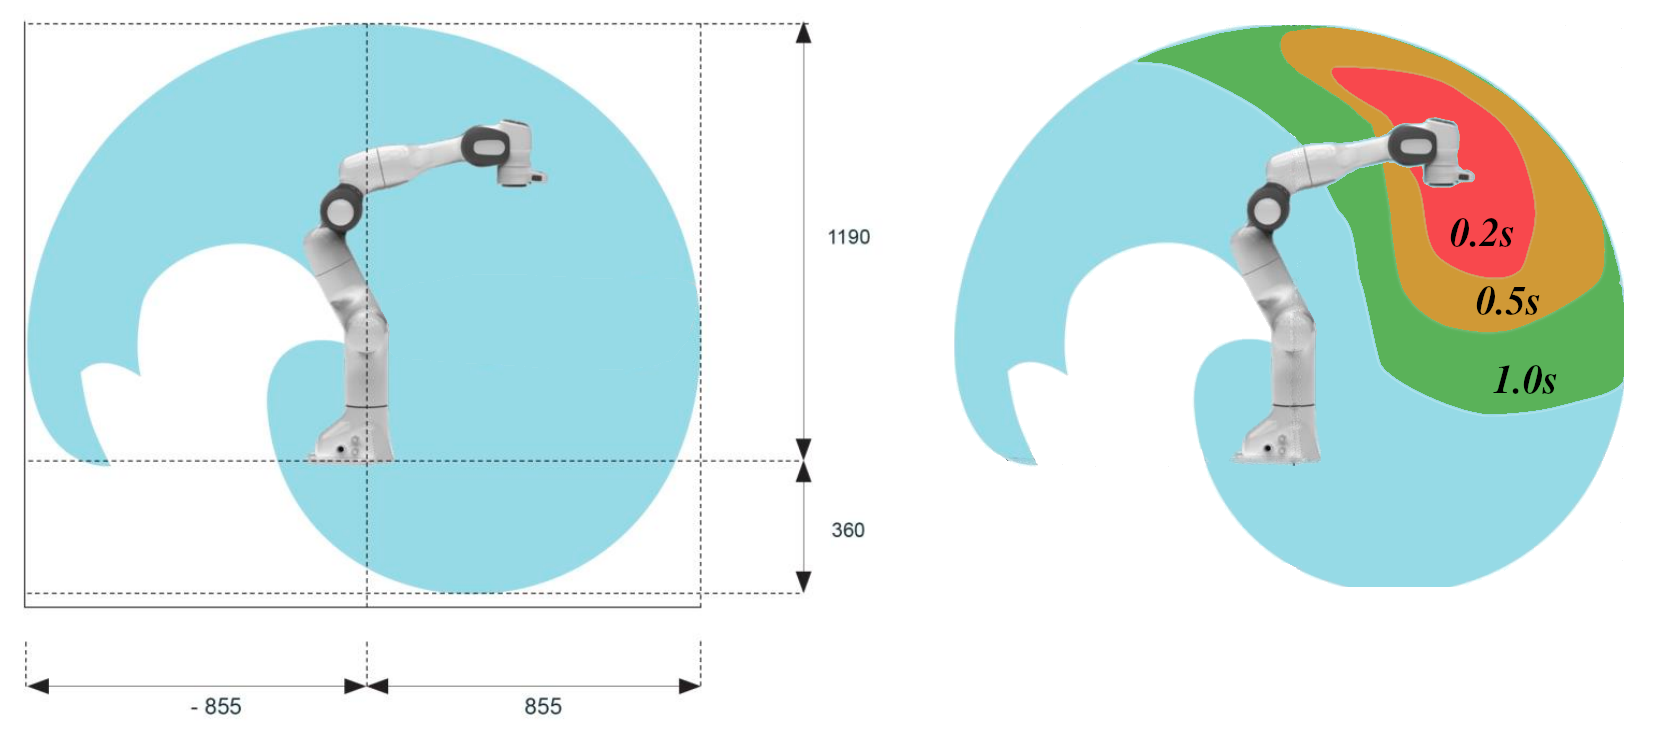
\includegraphics[width=0.8\linewidth]{Papers/images/all_rs_thesis.png}
    \caption{Figure on the left shows a section of the reachable workspace for a Franka Emika Panda robot given in the manufacturer's datasheet \cite{franka_maual}, as the area shown in blue. Figure on the right conceptually illustrates, in different colours, the area of this workspace reachable within the horizon times of $0.2$s, $0.5$s and $1$s.}
    \label{fig:franak_reachable_worksapce}
\end{figure}

As robotic systems are highly nonlinear and featuring complex kinematics and dynamics, the exact characterisation of their reachable spaces is very complex to characterise and calculate. Therefore, approximation techniques are necessary in order to yield practical solutions \cite{Althoff2021SetBased}. \citet{pereira2017} have developed an set based approach, later improved by \citet{schepp2022}, to approximate the human arm reachable space, modelled as a serial robotic manipulator. Their approach approximates the reachable space using a set of spheres and cylinders. However, in many cases the approximation of the reachable space using these shapes is impractical sue to their nonlinear nature. 

In this section, an approximation approach of the robot's reachable space using convex polytopes is proposed, leveraging several of their key characteristics. Since the reachable space is often low dimensional ($\leq$3D) these polytopes can be easily visualised, having the structure of a triangulated mesh. Additionally, convex polytopes can be represented as a set of linear inequalities $A\bm{x}\leq\bm{b}$, which may be directly used with different optimisation techniques. Additionally, this set of linear inequalities can be intuitively extended with different environmental and user defined constraints. Furthermore, operations over polytopes such as Minkowski sum and intersection are well defined and efficient to calculate, enabling for the intuitive extension of the proposed method to account for robot's link geometry. Finally, the efficiency of polytope enumeration techniques for low dimensional polytopes has a potential to make this metric real-time capable. 

As discussed in \Cref{ch:phisical_ability_metrics}, convex polytopes are widely used to characterise different task space physical abilities in robotics (ex. force, acceleration, velocity capacity). However, to the best of our knowledge they have not yet been used to characterise the reachable space of a robotic manipulator. The proposed approach is partially inspired by the works of \citet{Long2018Evaluating} on the constrained manipulability (velocity) polytopes.  

The section has the following structure. In \Cref{ch:polytope} the formal definition of the approach is introduced, as well as its extension with the environmental constraints and the link geometry. \Cref{ch:analysis} brings the analysis of the accuracy of the convex polytope approximation, as well as the execution time analysis. In \Cref{ch:results}, the results of the accuracy and execution time analysis of the approach are given and \Cref{ch:discussion} brings the discussion on main limitations.


\subsection{Reachable space polytope definition}
\label{ch:polytope}

The dynamics equation of a serial robot in \gls{js} can be expressed as
\begin{equation}
    M(\bm{q})\ddot{\bm{q}} +\underbrace{ C(\bm{q},\dot{\bm{q}})\dot{\bm{q}} + \bm{g}(\bm{q}) }_{\bm{\tau}_d}= \bm{\tau}
    \label{eq:robot_model}
\end{equation}
where $M\in\mathbb{R}^{n\times n}$ is the mass matrix, $C\in\mathbb{R}^{n\times n}$ is a matrix grouping Coriolis and centrifugal effects and $\bm{g}\in\mathbb{R}^{n}$ is the gravity vector. $\bm{\tau}\in\mathbb{R}^{n}$ is the applied joint torque vector and $\bm{\tau}_d\in\mathbb{R}^{n}$ is the equivalent joint torque vector due to the nonlinear effects of the robot's movement and gravity. Vectors $\bm{q},\dot{\bm{q}},\ddot{\bm{q}}\in\mathbb{R}^n$ are robot's \gls{js} position, velocity and acceleration respectively.

For a robot with $n$ actuated degrees of freedom (DOF), the robot's joint torque $\bm{\tau}$, velocity $\dot{\bm{q}}$ and joint angles $\bm{q}$ are $n$-dimensional vectors, limited by the robot's hardware\footnote{There is a coupling between the velocity and torque limits of an actuator related to its power. Yet, it is common practice to consider a subset of these limits such as torque and velocity can be chosen independantly one from the other.}
\begin{equation}
 \bm{\tau}\in\left[\bm{\tau}_{min},\bm{\tau}_{max}\right], \quad 
 \dot{\bm{q}}\in\left[\dot{\bm{q}}_{min},\dot{\bm{q}}_{max}\right], \quad \bm{q}\in\left[\bm{q}_{min},\bm{q}_{max}\right]
 \label{eq:limits}
\end{equation}


For a given moment in time $t_o$ and corresponding robot's state $\{\bm{q}_o,\dot{\bm{q}}_o\}$, the affine relationship between joint torques $\bm{\tau}$ and accelerations $\ddot{\bm{q}}_{o}$ can be expressed as
\begin{equation}
    \ddot{\bm{q}}_{o} = M^{-1}(\bm{q}_o)(\bm{\tau} - \bm{\tau}_d(\bm{q}_o,\dot{\bm{q}}_o)) = M_o^{-1}(\bm{\tau} - \bm{\tau}_{d,o})
\end{equation}

Considering a constant joint acceleration $\ddot{\bm{q}}_{o}$ during a given horizon length $t_h$, an approximation of the robot's joint velocity $\dot{\bm{q}}_{h}$ and position $\bm{q}_{h}$, at the end of horizon, can be calculated using numerical integration (forward Euler method) 
\begin{equation}
    \dot{\bm{q}}_{h} = M_o^{-1}t_h(\bm{\tau} - \bm{\tau}_{d,o}) + \dot{\bm{q}}_{o}, \qquad \bm{q}_{h} = M_o^{-1}\frac{t_h^2}{2}(\bm{\tau} - \bm{\tau}_{d,o}) + \dot{\bm{q}}_{o}t_h + \bm{q}_{o}
    \label{eq:joint_vel_pos}
\end{equation}
This linear numerical integration (\ref{eq:joint_vel_pos}) considers the robot's dynamics (\ref{eq:robot_model}), and the applied joint torque $\bm{\tau}$, fixed during the horizon time $t_h$. Such assumption is reasonable only for short horizon times $t_h$ which in term represents a limitation of the proposed method.

The relationship between the $m$-dimensional task space velocity $\dot{\bm{x}}$ and acceleration $\ddot{\bm{x}}$ of certain frame on the robot (for example end-effector frame) and the $n$-dimensional \gls{js} equivalents is defined through the corresponding Jacobian matrix $J(\bm{q})\in\mathbb{R}^{m\times n}$ and its time derivative $\dot{J}(\bm{q})\in\mathbb{R}^{m\times n}$
\begin{equation}
    \dot{\bm{x}} = J \dot{\bm{q}}, \qquad  \ddot{\bm{x}} = J \ddot{\bm{q}} + \dot{J} \dot{\bm{q}}
\end{equation}

Finally, given the horizon of interest $t_h$, the predicted \gls{cs} position $\bm{x}_{h}$ can then be expressed as

\begin{equation}
\begin{split}
    {\bm{x}}_{h} &= \ddot{\bm{x}}_o\frac{t_h^2}{2}   \qquad\qquad\qquad\qquad\qquad\qquad\qquad\qquad+\dot{\bm{x}}_ot_h \quad +\!  \bm{x}_o\\
    &=  J_o M_o^{-1}\frac{t_h^2}{2}\bm{\tau} \quad \underbrace{\underbrace{-
    J_o M_o^{-1}\frac{t_h^2}{2}\bm{\tau}_{d,o}}_{\Delta \bm{x}_{o,dyn}}  \quad \underbrace{ +\dot{J}_o \dot{\bm{q}}_o\frac{t_h^2}{2} \quad+ \dot{\bm{x}}_ot_h}_{\Delta \bm{x}_{o,vel}} \quad + \bm{x}_{o} }_{\hat{\bm{x}}_{h}}
    \end{split}
    \label{eq:pred_pos}
\end{equation}

Where $\hat{\bm{x}}_{h}\! =\!\Delta \bm{x}_{o,dyn}\! +\! \Delta \bm{x}_{o,vel} + \bm{x}_{o}$ is a predicted position vector calculated by integrating the influences of the robot's joint movement $\{\dot{\dot{\bm{q}}}_o,\bm{\tau}_{d,o}\}$ over the time horizon $t_h$. The first term describes the influence of the applied joint torques $\bm{\tau}$ on \gls{cs} position reached, considered constant during the horizon $t_h$.

The convex polytope of reachable \gls{cs} positions $\mathcal{P}_x$ can then be defined as a set of all the possible \gls{cs} positions $\bm{x}_{h}$ at the end of the horizon $t_h$, achieved by any combination of joint torques $\bm{\tau}$ within robot's physical limitations (\ref{eq:limits}), given the robot's current state $\{\dot{\bm{q}}_o$, $\bm{q}_o\}$ and $\bm{\tau}_{d,o}$.
\begin{equation}
\begin{split}
    \mathcal{P}_x= \{ \bm{x}_{h} \in \mathbb{R}^m \quad| \quad \bm{x}_{h} &= J_o M_o^{-1}\frac{t_h^2}{2}\bm{\tau} + \hat{\bm{x}}_{h},\\
    \quad \bm{\tau} &\in \left[\bm{\tau}_{min},\bm{\tau}_{max}\right],\\
   M_o^{-1}t_h (\bm{\tau} - \bm{\tau}_{d,o}) + \dot{\bm{q}}_o &\in \left[\dot{\bm{q}}_{min},\dot{\bm{q}}_{max}\right],\\
   M_o^{-1}\frac{t_h^2}{2}(\bm{\tau} - \bm{\tau}_{d,o}) +  \dot{\bm{q}}_ot_h + \bm{q}_o &\in \left[\bm{q}_{min},\bm{q}_{max}\right] \}
\end{split} 
\label{eq:polytope_simple}
\end{equation}

Polytope $\mathcal{P}_x$ formulation (\ref{eq:polytope_simple}) can also be seen as projection of the joint torque polytope $\mathcal{P}_\tau$ to the lower $m$ dimensional task space
\begin{equation}
    \mathcal{P}_x= \{ \bm{x}_{h} \in \mathbb{R}^m ~| ~ \bm{x}_{h} = J_o M_o^{-1}\frac{t_h^2}{2}\bm{\tau} + \hat{\bm{x}}_{h},\quad \bm{\tau}\in\mathcal{P}_\tau\}
\end{equation}
where the joint torque polytope $\mathcal{P}_\tau$ integrates all the joint actuator limits (\ref{eq:limits}) of the robot
\begin{equation}
\begin{split}
    \mathcal{P}_\tau= \{ \bm{\tau} \in \mathbb{R}^n \quad|\qquad\qquad\qquad\qquad \bm{\tau} &\in \left[\bm{\tau}_{min},\bm{\tau}_{max}\right],\\~
   M_o^{-1}t_h (\bm{\tau} - \bm{\tau}_{d,o}) + \dot{\bm{q}}_o &\in \left[\dot{\bm{q}}_{min},\dot{\bm{q}}_{max}\right],\\
   M_o^{-1}\frac{t_h^2}{2}(\bm{\tau} - \bm{\tau}_{d,o}) +  \dot{\bm{q}}_ot_h + \bm{q}_o &\in \left[\bm{q}_{min},\bm{q}_{max}\right] \}
\end{split} 
\label{eq:torqe_poly_rs}
\end{equation}

\qrimg{qrcodes/reachable_space_convex_video_sim.png}{https://youtu.be/JwZgrUp095Y}{Video}
The visualisation potential of the proposed polytope formulation $\mathcal{P}_x$ is showcased on \Cref{fig:horizon}, \Cref{fig:limits}, and \Cref{fig:velocity}, as well as in the publicly available video\footnote{Video: \url{https://youtu.be/JwZgrUp095Y}}. The influences of the robot's actuator constraints, robot movement ($\dot{\bm{q}}_o,\bm{\tau}_{d,o}$) and different horizon lengths $t_h$, is captured through the changing shape and size of the reachable space polytope $\mathcal{P}_x$.

The following sections extend this polytope formulation with the carried payload, environmental constraints and the robot's link geometry. \Cref{ch:enumerating} then describes an efficient approach to finding the $\repr{H}$ and $\repr{V}$-representation of the reachable space polytope $\mathcal{P}_x$. 


\begin{figure}[!h]
    \centering
    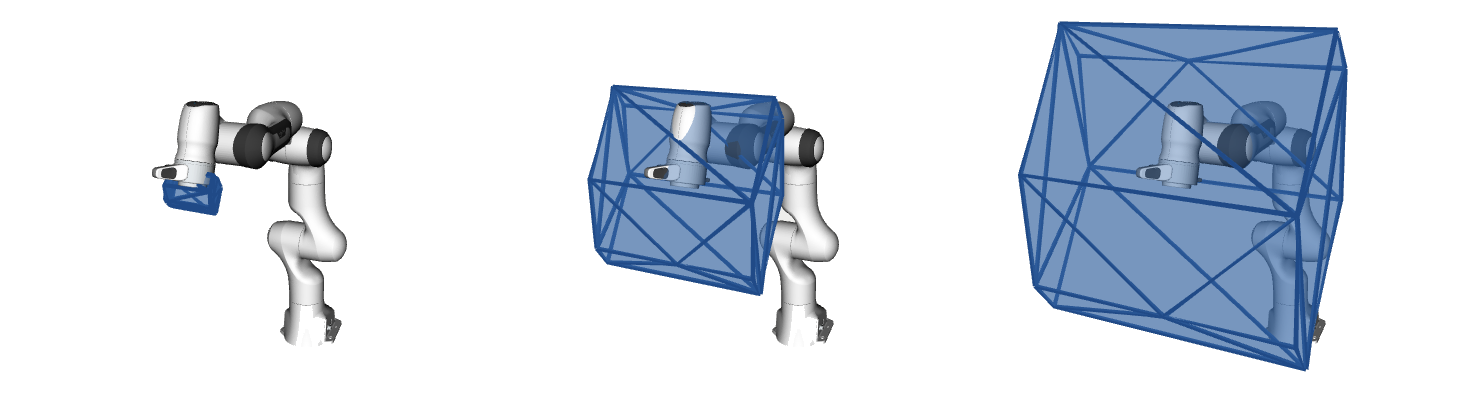
\includegraphics[width=\linewidth]{Papers/images/horizon.png}
    \caption{Three images show the comparison of the size of the reachable space polytope $\mathcal{P}_x$ of a Franka Emika Panda\protect\footnotemark ~~robot's end-effector for 3 horizons  (left to right) $t_h$ = 0.05, 0.15 and 0.25s, for the same configuration. } 
    \label{fig:horizon}
\end{figure}
\footnotetext{More information about the Panda robot at \url{https://frankaemika.github.io/docs/}}

\begin{figure}[!h]
    \centering
    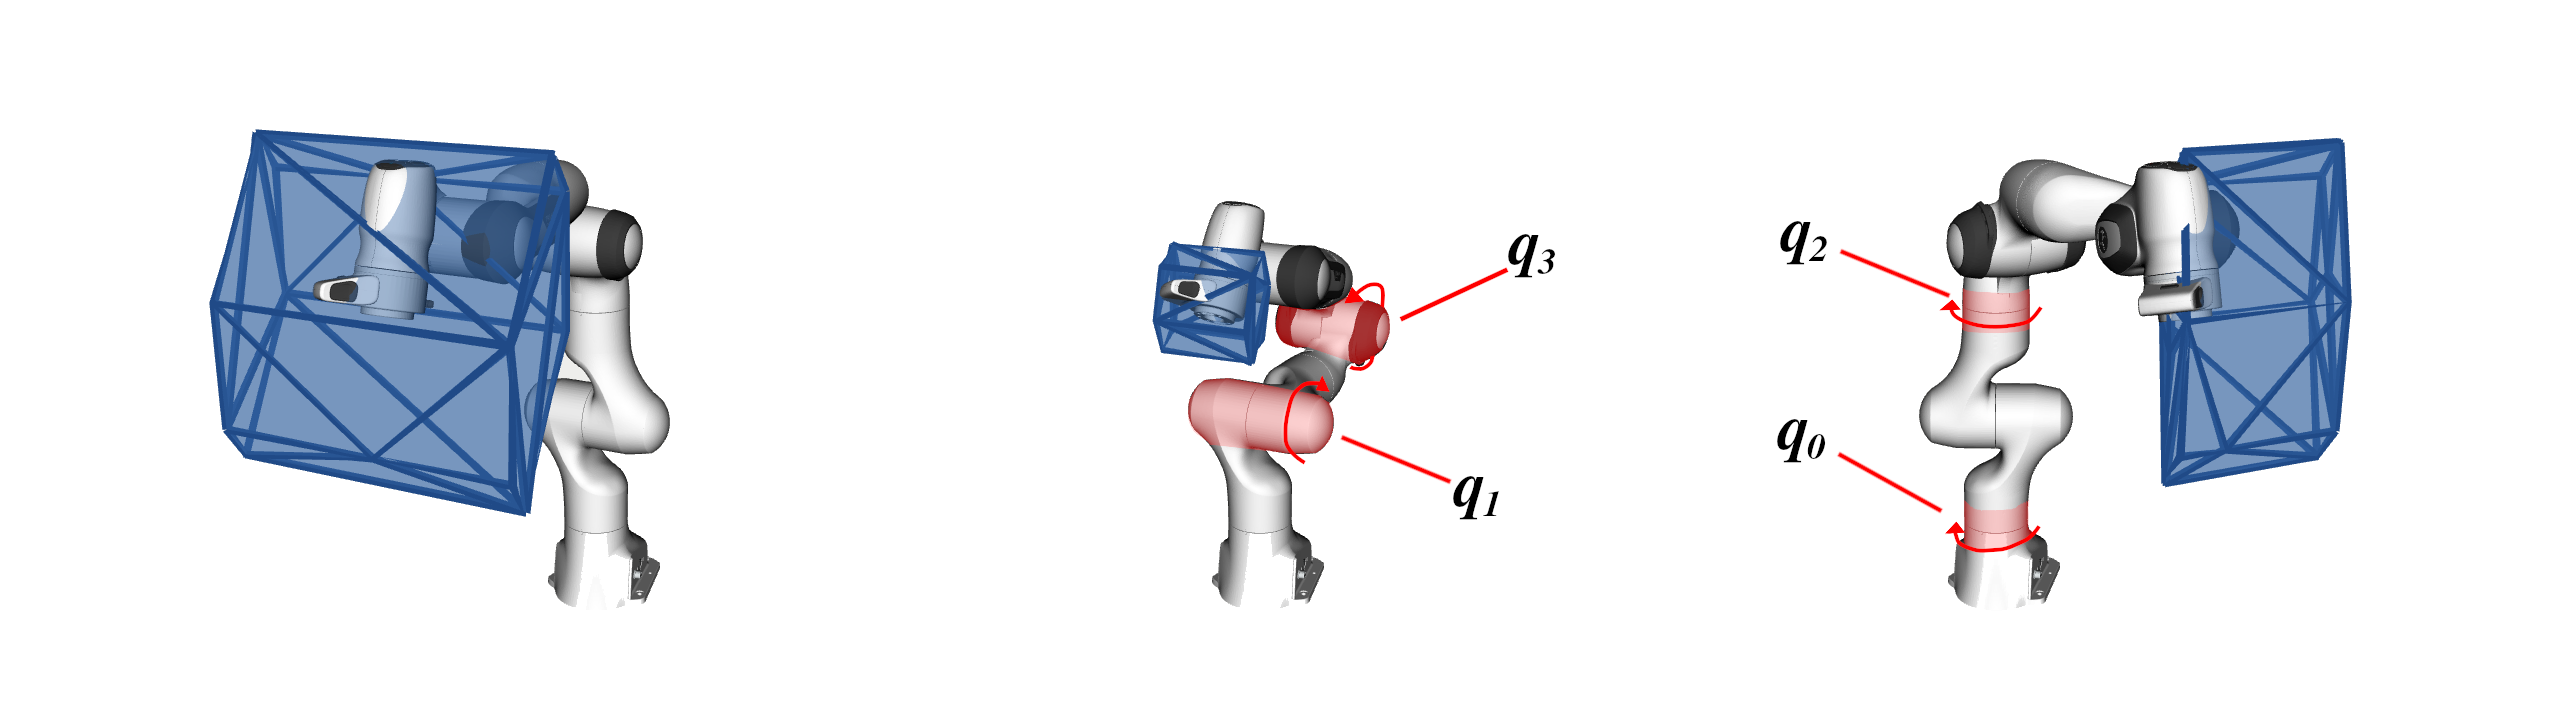
\includegraphics[width=\linewidth]{Papers/images/limits.png}
    \caption{Reachable space polytope $\mathcal{P}_x$ for a Franka Emika Panda robot's end-effector for 3 configurations ($t_h$=0.15s). On the left, the robot is in its initial position $\bm{q}=[0,0,0,-\pi/2, 0, 3\pi/5,0]$, close to the center of the joint ranges. 
    In the middle figure the robot has joints $q_1$ and $q_3$ are at their limits, $\bm{q}=[0,-1.59,0,-2.9,0,3\pi/5,0,0]$. 
    On the right, robot's joints $q_0$ and $q_2$ are at their limits $\bm{q}=[-2.72,0, -2.72,-\pi/2,0,13\pi/5,0,0]$, preventing the robot to rotate around the z axis in one direction.
    }
    \label{fig:limits}
\end{figure}

% \begin{figure}[!t]
%     \centering
%     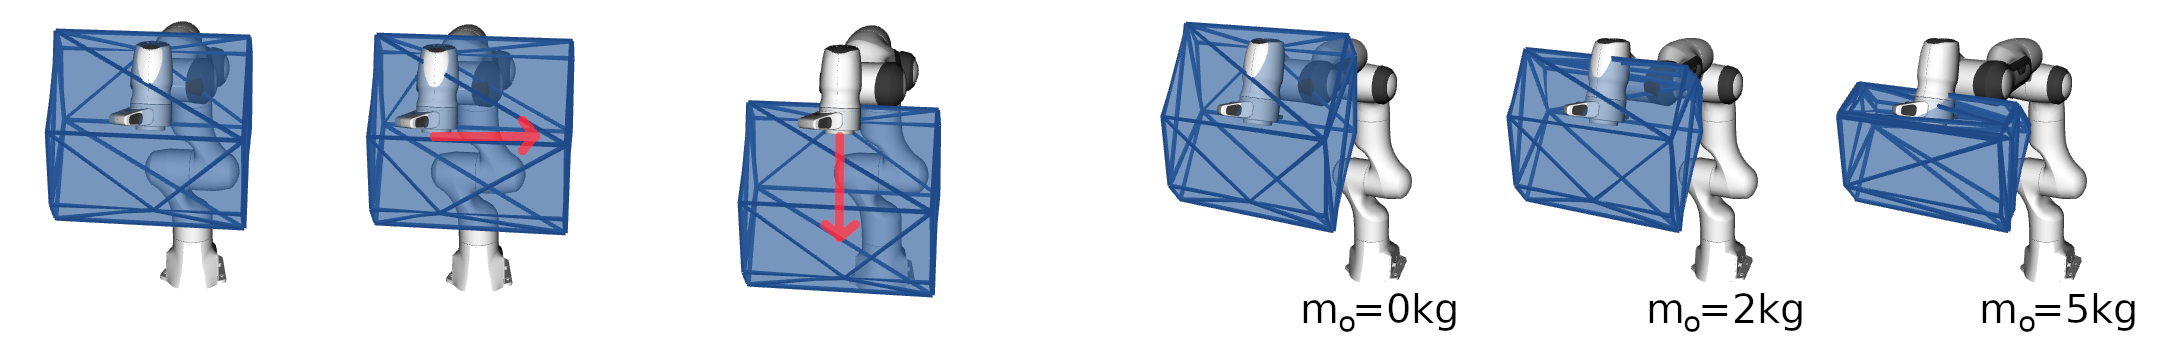
\includegraphics[width=\linewidth]{Papers/images/vel_object.png}
%     \caption{Three images on the left show the shifting effect on the reachable space polytope $\mathcal{P}_x$ produced by certain \gls{cs} velocity at the beginning of the horizon, from left to right: $\dot{\bm{x}}_k$ = $[0,0,0]$, $[0,1,0] $ and $[0,0,-1]m/s$. Three images on the right show the reducing effect on the polytope $\mathcal{P}_x$ by three different carried object masses (left to right) $m_o$ = 0, 2 and 5kg. Horizon used is $t_h$=0.15s and the robot is in initial configuration.}
%     \label{fig:velocity}
    
% \end{figure}

\begin{figure}[!h]
    \centering
    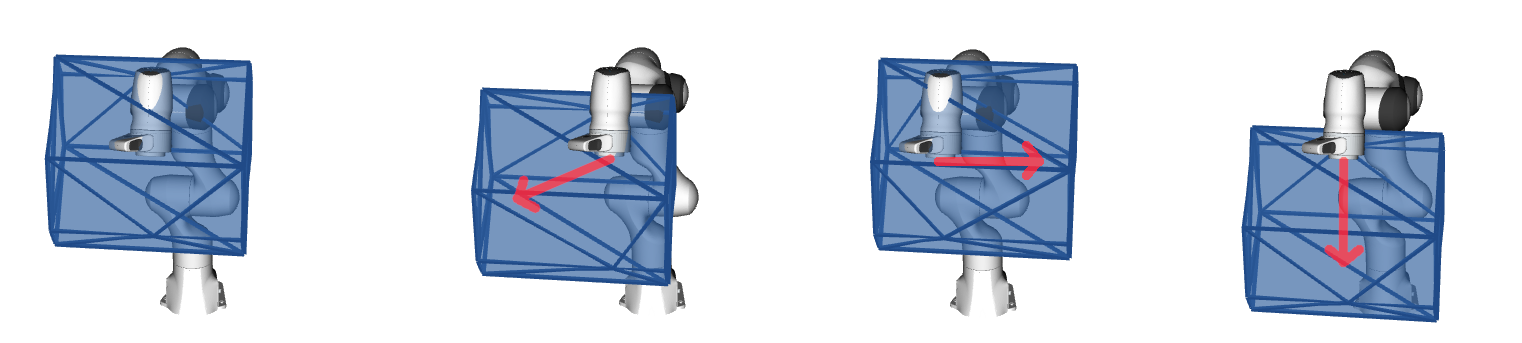
\includegraphics[width=\linewidth]{Papers/images/vel.png}
    \caption{Reachable space polytope $\mathcal{P}_x$ for a Franka Emika Panda robot's end-effector for 4 different end-effector velocities $\dot{\bm{x}}_o\!=\!J\dot{\bm{q}}_o$ (from left to right) $\dot{\bm{x}}_o$ = $[0,0,0]$, $[0,-1,-0.5]$, $[0,1,0] $ and $[0,0,-1]m/s$.}
    \label{fig:velocity}
\end{figure}

\begin{figure}[!h]
    \centering
    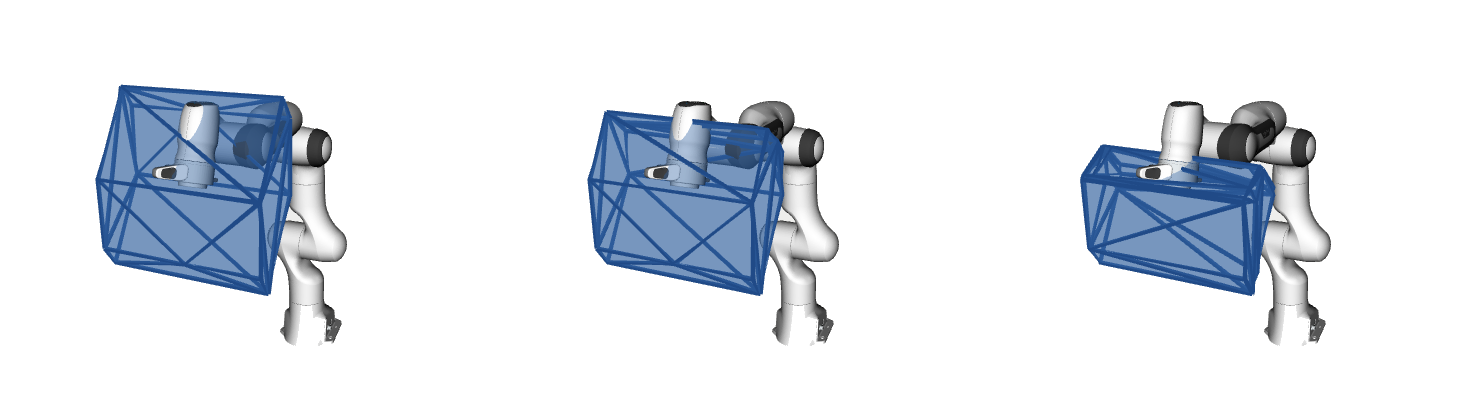
\includegraphics[width=\linewidth]{Papers/images/object.png}
    \caption{Reachable space polytope $\mathcal{P}_x$ for a Franka Emika Panda robot for three different carried object masses (left to right) $m_{object}$ = 0, 2 and 5kg, horizon time used $t_h$=0.15s.}
    \label{fig:objectt}
\end{figure}

\subsubsection{Influence of the carried object}

Consider a robot that carries a payload, an object with a mass $m_{object}$ and inertia $i_{object}$, attached to its end-effector. This object has an influence on the robot's dynamics, modifying the mass matrix $M$, coriolis matrix $C$ and the gravity vector $\bm{g}$ \cite{hamad2019}.
The augmented dynamical model of the robot has reduced acceleration capabilities due to the added effort necessary for the object's movements.


\Cref{fig:objectt} shows the influence of different object masses $m_{object}$, on the resulting reachable space polytope $\mathcal{P}_x$ for the {Franka Emika Panda} robot. 

\subsubsection{Integration of the environment}

\begin{figure}[!b]
    \centering
    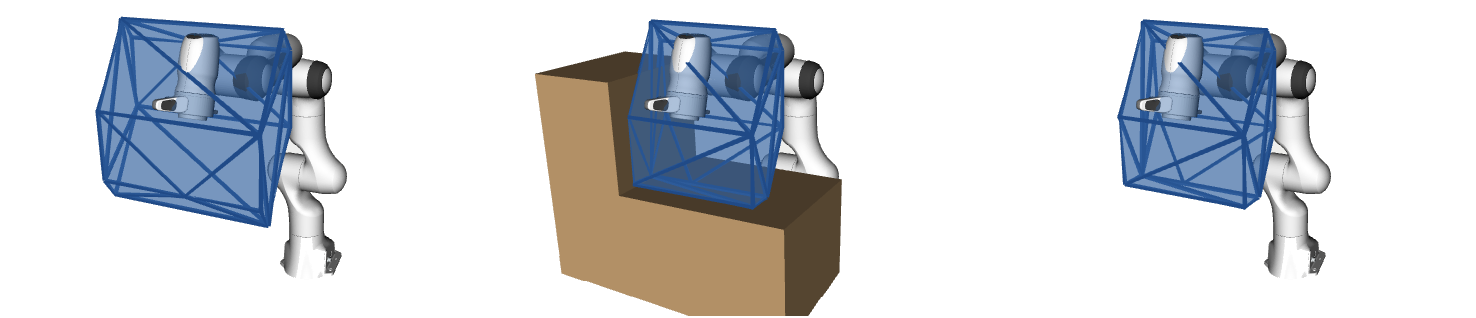
\includegraphics[width=\linewidth]{Papers/images/env1.png}
    \caption{Resulting reachable space polytope $\mathcal{P}_x$ for a Franka Emika Panda robot's end-effector when integrating the environmental constraints, horizon time used is $t_h$=0.15s. Environment is defined as $z\geq0.5$m and $y\geq-0.2$m.}
    \label{fig:env}
    
\end{figure}

If the robot's environment can be defined as a set of convex inequalities
\begin{equation}
    A_e \bm{x} \leq b_e
\end{equation}
these constraints can be directly transformed to the constraints of the joint torque $\bm{\tau}$ using the equation (\ref{eq:pred_pos})
\begin{equation}
    A_e\bm{x}_{h} = A_e J_o M_o^{-1}\frac{t_h^2}{2} \bm{\tau}  + A_e \hat{\bm{x}}_{h} \leq b_e
    \label{eq:env_limits}
\end{equation}
and then included in the $\mathcal{P}_x$ calculation (\ref{eq:polytope_simple})
\begin{equation}
\begin{split}
    \mathcal{P}_x= \{ \bm{x}_h \in \mathbb{R}^m \quad| \quad \bm{x}_h &= J_o M_o^{-1}\frac{t_h^2}{2}\bm{\tau} + \bm{x}^*_h,\\
   \quad \bm{\tau} &\in \left[\bm{\tau}_{min},\bm{\tau}_{max}\right],\\
    M_o^{-1}t_h (\bm{\tau} -\bm{\tau}_{d,o})+ \dot{\bm{q}}_o &\in \left[\dot{\bm{q}}_{min},\dot{\bm{q}}_{max}\right],\\
   M_o^{-1}\frac{t_h^2}{2}(\bm{\tau} -\bm{\tau}_{d,o}) +  \dot{\bm{q}}_ot_h + \bm{q}_o &\in \left[\bm{q}_{min},\bm{q}_{max}\right],\\
   A_e J_o M_o^{-1}\frac{t_h^2}{2} \bm{\tau}  + A_e \bm{x}^*_h &\leq b_e ~~\}
\end{split} 
\label{eq:env}
\end{equation}

\Cref{fig:env} showcases the extension of the reachable space polytope $\mathcal{P}_x$ with the environmental constraints, influencing directly its shape. The same approach can be used to visualise the robot's task space constraints to the operator, enforced by the robot control. For example in the case of robot teleoperation, the polytope $\mathcal{P}_x$ can be used to visualise to the operator the space reachable by the robot while including virtual walls \cite{Colgate1996Cobots}.




\subsubsection{Integration of robot's link geometry}

Leveraging the efficient tools from polytope algebra, the proposed reachable space approximation can be extended to the calculation of the reachable space of robot's links as well.

For example, if a robot link $l_i$ is modelled as a line segment, the polytope $\mathcal{P}_x$ can be calculated at the start $\mathcal{P}_{xs}$ and the end $\mathcal{P}_{xe}$ of the line $l_i$. Then, the reachable space of this idealised robot link $l_i$ can then be calculated as the Convex-Hull ($\conv{\cdot}$) of the polytopes $\mathcal{P}_{xs}$ and $\mathcal{P}_{xe}$
\begin{equation}
    \mathcal{P}_{x,l_i} = \conv{  \mathcal{P}_{xs}, ~ \mathcal{P}_{xe}}
\end{equation}
\Cref{fig:minkowski_line} shows the construction of  the reachable space polytope of the Panda robot's link 3, modelled as a line segment.

If, instead of a straight line, a space captured by a robot's link $l_i$ can be expressed as a convex set of constraints or a polytope ($\repr{H}$-representation)
\begin{equation}
    \mathcal{L}_i = \Big \{ \bm{x}_{l_i} ~ |~ A_{l_i} \bm{x}_{l_i} \leq b_{l_i} \Big\}
\end{equation}
the reachable space polytope $\mathcal{P}_{x,l_i}$ can be extended to account for this link geometry by first finding the vertices ($\repr{V}$-representation) of the polytope $\mathcal{L}_i$, for example using one of the standard polytope transformation methods described in \Cref{ch:standard_represtantion_conversion}. Then the reachable space polytope $\mathcal{P}_{x}$ can be evaluated for each one of the $N_v$ vertices, while the full link polytope $\mathcal{P}_{x,\mathcal{L}_i}$ can be found by computing their Convex-Hull
\begin{equation}
    \mathcal{P}_{x,\mathcal{L}_i} = \conv{  \mathcal{P}_{x1}, ~ \dots ~, \mathcal{P}_{xN_v} }
\end{equation}

\qrimg{qrcodes/reachable_space_convex_body_video_sim.png}{https://youtu.be/1J2UrMC2uP0}{Video}
By evaluating the polytope $\mathcal{P}_{x,\mathcal{L}_i}$ for each robot's link one can obtain an efficient approximation of the reachable space of the entire robot. One example of constructing such reachable space is shown on \Cref{fig:minkowski_block}.

The link polytopes $\mathcal{P}_{x,\mathcal{L}_i}$ can be further used to calculate the convex envelope $\mathcal{P}_{env}$ of the robot's reachable space as well, by calculating the their Convex-Hull.
\begin{equation}
    \mathcal{P}_{env} = \conv{  \mathcal{P}_{x,\mathcal{L}_1},~ \mathcal{P}_{x,\mathcal{L}_2}, ~ \dots ~ }
\end{equation}
An interactive visualisation of the reachable space approximation for the robot's links as well as its convex envelope can be found in the publicly available video\footnote{Video: \url{https://youtu.be/1J2UrMC2uP0}}.

\begin{figure}[!t]
    \centering
    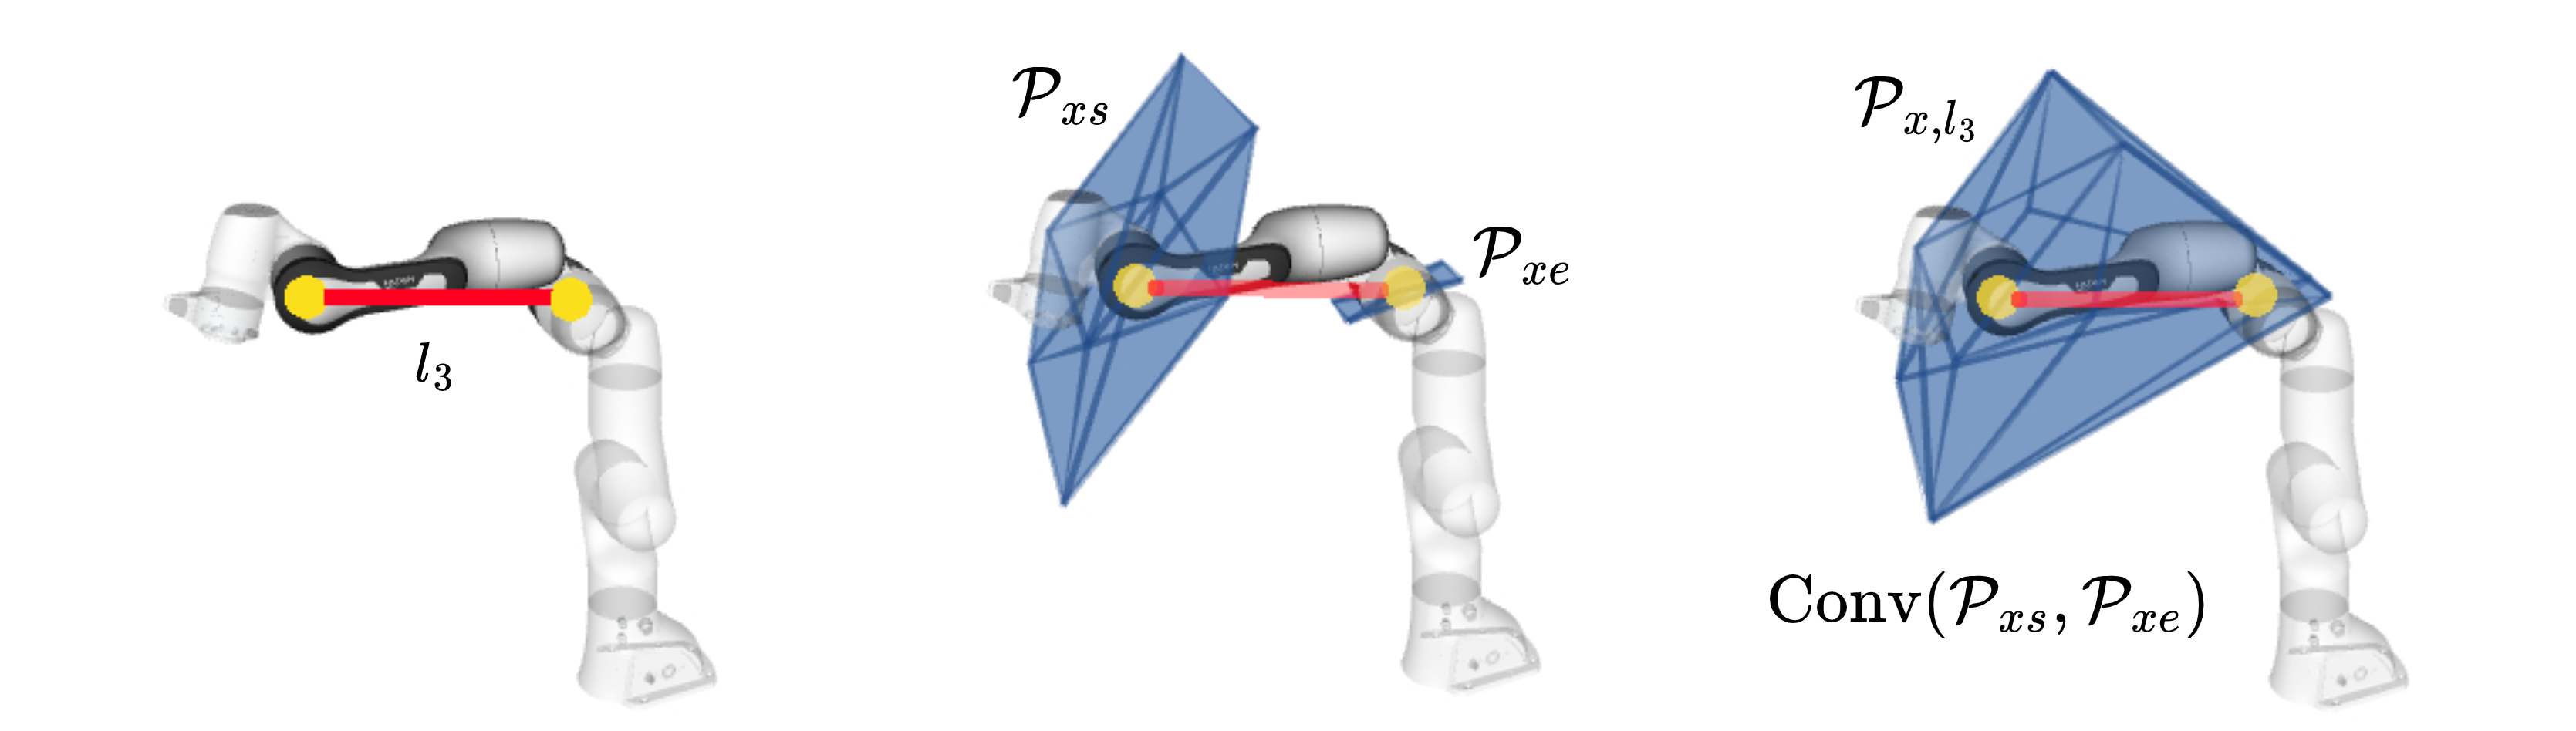
\includegraphics[width=0.8\linewidth]{Papers/images/minkowski_line_nomath_withmath.png}
    \caption{ The figure shows the construction of the reachable space polytope of the Panda robot's link 3, $\mathcal{P}_{x,l_3}$. The first image shows the robot's link 3 modelled as a line segment $l_3$ (in red). The polytopes $\mathcal{P}_{xs}$ and $\mathcal{P}_{xe}$ calculated in its vertices (yellow) are shown in the middle. $\mathcal{P}_{x,l_3}$, calculated as their Convex-Hull, is shown on the right. Robot is in its initial configuration, and the horizon time used is 150ms.}
    \label{fig:minkowski_line}
\end{figure}

\begin{figure}[!t]
    \centering
    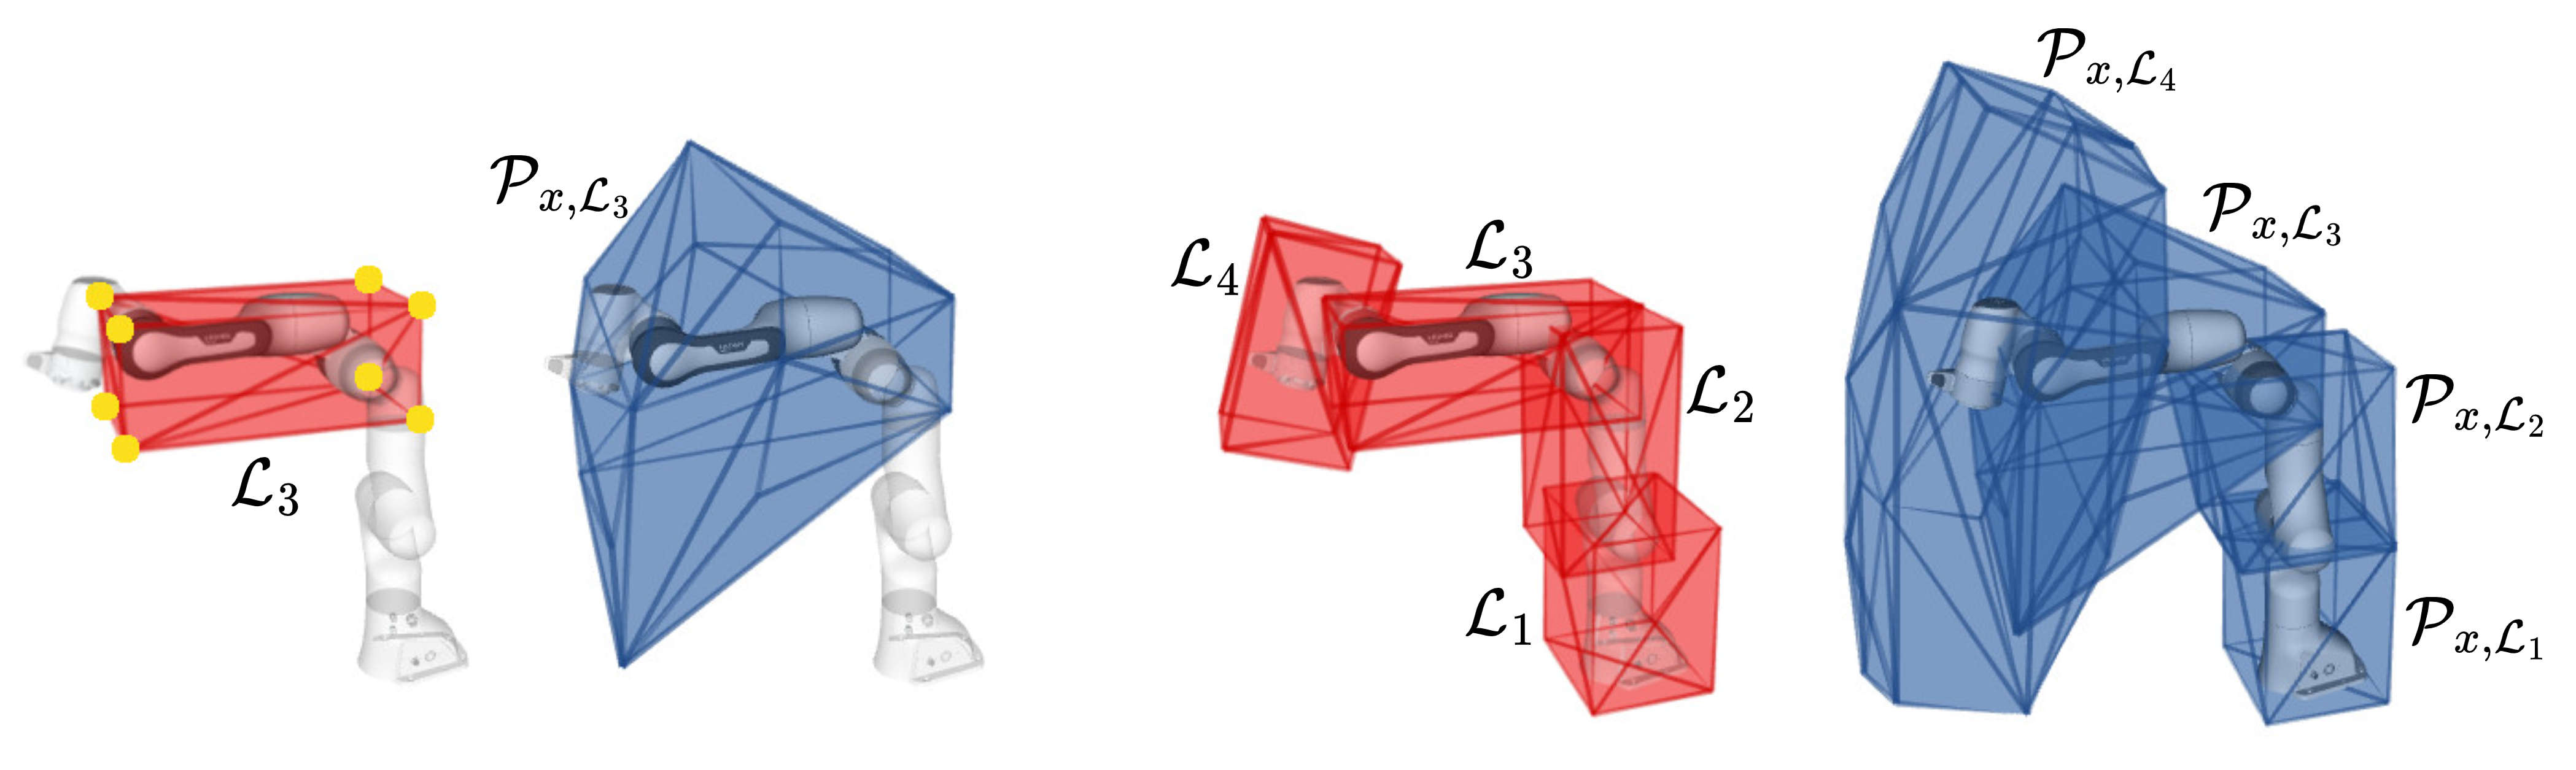
\includegraphics[width=\linewidth]{Papers/images/minkowski_block_nomath_withmath.jpg}
    \caption{ First two images show the construction of the reachable space polytope of the panda robot's link 3, $\mathcal{P}_{x,\mathcal{L}_3}$. The left figure shows the link 3 $\mathcal{L}_3$, modelled as a box (in red). Followed by the visualisation of its reachable space polytope $\mathcal{P}_{x,\mathcal{L}_3}$, calculated as a Convex-Hull of the polytopes of each one of its 8 vertices (in yellow).
    Last two images show 4 enveloping spaces $\mathcal{L}_i$ for each one of the robot's links, and their reachable space polytopes $\mathcal{P}_{x,\mathcal{L}_i}$. Robot is in its initial configuration, and the horizon time used is 150ms.}
    \label{fig:minkowski_block}
\end{figure}


\subsection{Finding $\repr{H}$ and $\repr{V}$-representation of the reachable space polytope}
\label{ch:enumerating}

In order to be used with standard applications, such as to be visualised to the operator, this polytope has to be transformed to the set of the vertices ($\repr{V}$-representation) or the set of half-planes ($\repr{H}$-representation) representing its faces.

The reachable space polytope $\mathcal{P}_x$ belongs to the family of problems
\begin{equation}
    \mathcal{P}_x = \{ \bm{x} \in \mathbb{R}^m \quad| \quad \bm{x}=B\bm{\tau} + \bm{b}_x,\quad  H_\tau\bm{\tau}\leq \bm{d}_\tau ~~\}, \quad \bm{\tau}\in \mathbb{R}^n, \quad n\geq m
\label{eq:polytope_family}
\end{equation}
where the inequality constraint $H_\tau\bm{\tau}\leq \bm{d}_\tau$ encapsulates all the robot constraints (\ref{eq:limits}) as well as the environmental constraints (\ref{eq:env_limits}), and the matrix $J_o M_o^{-1}\frac{t_h^2}{2}$ becomes the projection matrix $B$. Vector $\bm{\tau}$ corresponds to the joint torque vector, $\bm{x}$ corresponds to the positions at the end of the horizon $\bm{x}_{h}$ and the bias vector $\bm{b}_x$ corresponds to $\hat{\bm{x}}_{h}$. 

This polytope has the projection formulation with polytope input set, as described in \Cref{ch:proj_formulaiton}. The set of constraints $H_\tau\bm{\tau}\leq\bm{d}_\tau$ forms a $\repr{H}$-representation of a polytope $\mathcal{P}_\tau$ in the $n$-dimensional joint torque space
\begin{equation}
    \mathcal{P}_\tau = \{ \bm{\tau} \in \mathbb{R}^n \quad| \quad H_\tau\bm{\tau}\leq \bm{d}_\tau ~~\}
\label{eq:polytope_torque}
\end{equation}
This polytope is then projected to the, usually much lower dimensional ($m\leq3$), \gls{cs}, forming the reachable space polytope $\mathcal{P}_x$ (\ref{eq:polytope_family}). 

As described more in detail in \Cref{ch:projection_algos}, and condensed in \Cref{tab:algorithms_table}, there are multiple ways to find the vertices and faces of this polytope. 
\Cref{tab:algorithms table} shows that if finding the $\repr{H}$-representation of the polytope $\mathcal{P}_x$, the most straight-forward methods are the \gls{fme}\cite{dantzig1973fourier} or \gls{esp}\cite{jones2004equality}. However, when searching for its $\repr{V}$-representation, no standard exact method can be directly applied. As described in \Cref{ch:proj_algos_v}, finding the $\repr{V}$-representation requires different multi-step approaches. 

In order to avoid using the multi-step approaches and to find both the $\repr{H}$ and $\repr{V}$-representations of the polytope $\mathcal{P}_x$ at the same time, Iterative Convex-Hull Method (ICHM) is used. ICHM method, described in detail in \Cref{ch:algorihtm_ichm}, is defined for a generic family of sets
\begin{equation}
\mathcal{P} = \{ ~\bm{x}\in \mathbb{R}^{m} ~|~ A\bm{x} = B\bm{y} + \bm{b},\quad H_y\bm{y} \leq \bm{d}_y~\}
\end{equation}
Using the ICHM algorithm for enumerating the reachable space polytope is rather straight-forward, by setting its matrix $A$ to identity $A=I_{m \times m}$, matrix $B$ becomes the projection matrix $P$, the inequality constraint $H_y\bm{y} \leq \bm{d}_y$ then becomes the set of the constraints $H_\tau\bm{\tau}\leq\bm{d}_\tau$ and the bias $\bm{b}$ becomes the bias $\bm{b}_x$.


\subsection{Analysing the approximation performance}
\label{ch:analysis}

The aim of the proposed polytope approximation of the robot's reachable space is to provide the real-time insight to the operators into the robot's state and its current physical abilities. 
Nevertheless, as this approach relies on approximating the actual reachable space, 
the accuracy of information provided to operators requires further validation. 
This section, therefore, brings a numerical analysis of the proposed approximation method's accuracy. 

Defining metrics of interest for accuracy analysis is highly dependent of the applications these methods will be used on. If the application requires an under-approximation of the reachable set or an over-approximation, the metrics of interest will not be the same. In this section, the proposed polytope accuracy is analysed using three different quantitative metrics, each one providing an insight in different characteristics and limitations of the method. 

Additionally, as this approximation method has a potential to be used for real-time applications, execution time analysis is performed as well. 

In the extent of the proposed experiments, the considered reachable space is the reachable space of the robot's end effector. 

\subsubsection{Numerical analysis of the approximation accuracy}

\begin{figure}[!h]
    \centering
    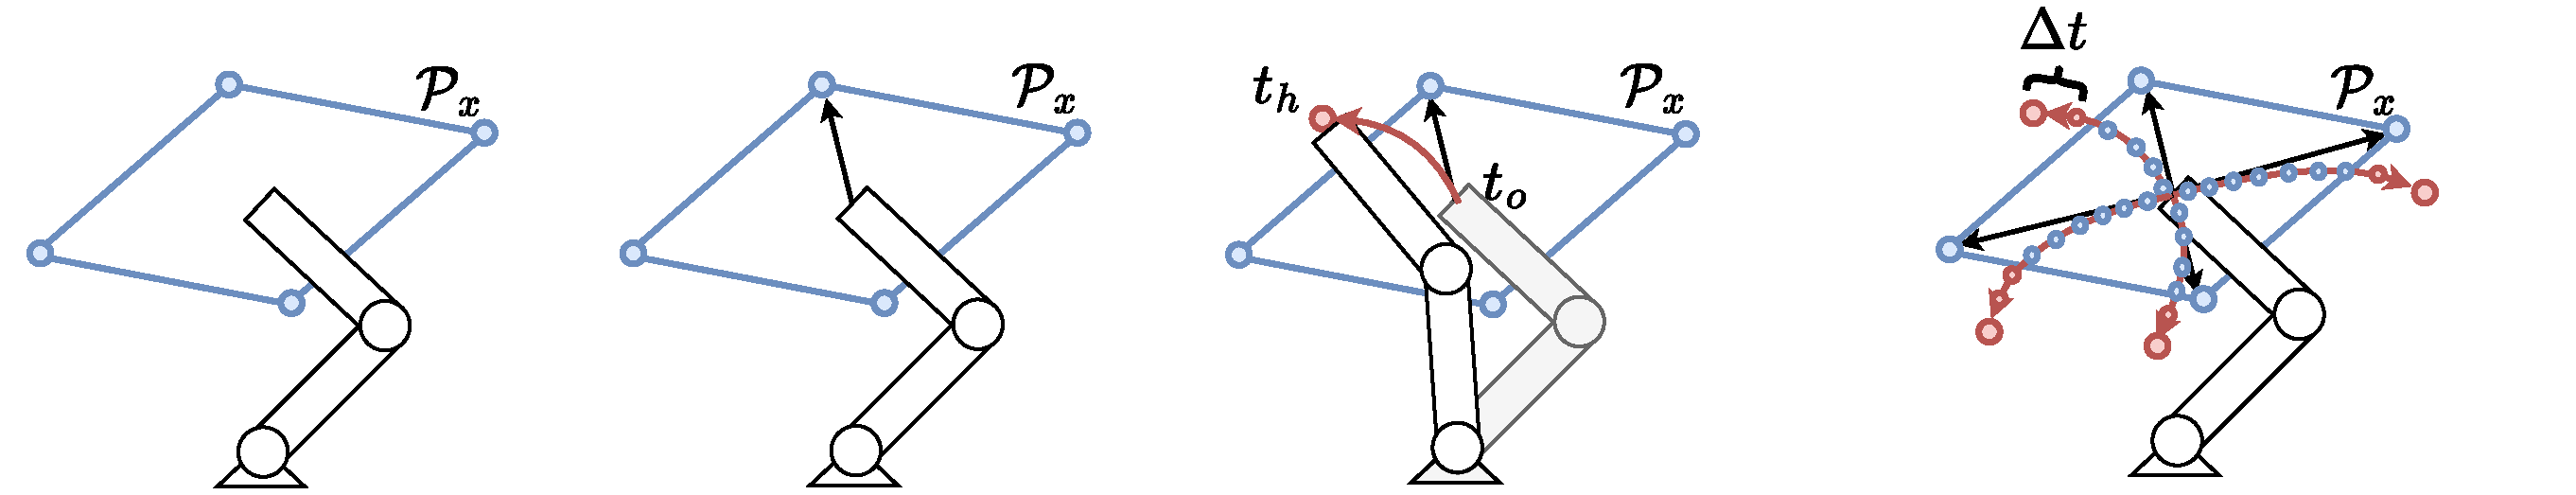
\includegraphics[width=\linewidth]{Papers/images/simulation.pdf}
    \caption{Images show the steps (left to right) of the nonlinear simulation procedure on a simplified 2 link planar robot. First the polytope $\mathcal{P}_x$ of the end-effector is determined. For each $\bm{x}_{v_i}$ vertex of the $\mathcal{P}_x$, the joint torque $\bm{\tau}_{v_i}$, generating this vertex, is applied to the robot simulation (figures in the middle). All the robot's end-effector positions $\bm{x}_k$ in all the simulation time steps $\Delta t$ are saved for further analysis.}
    \label{fig:simulation}   
\end{figure}
The main limitation of the proposed convex polytope $\mathcal{P}_x$ approach to the approximation of the robot's reachable space, and its main source of the approximation error, is the consideration of  robot's dynamics and kinematics to be linear.
Therefore, to analyse the approximation accuracy of the proposed approach, it is compared to the robot's nonlinear simulation.

Each vertex $\bm{x}_{v_i}$ of the reachable space polytope $\mathcal{P}_x$, calculated for the robot's state $\{\bm{q}_o,\dot{\bm{q}}_o\}$, is generated by a certain joint torque vector $\bm{\tau}_{v_i}$, considered constant during the time horizon $t_h$.
%This joint torque vector $\bm{\tau}_i$ belongs to a subset of vertices of the joint torque polytope $\mathcal{P}_\tau$. 
% The set of joint torques $\bm{\tau}_i$, generating the vertices $\bm{x}_{v_i}$, can be determined at the polytope $\mathcal{P}_x$ evaluation. 
Assuming the linear robot model, the joint torques $\bm{\tau}_{v_i}$, generating the vertices $\bm{x}_{v_i}$, correspond to the subset of vertices of the joint torque polytope $\mathcal{P}_\tau$ (\ref{eq:torqe_poly_rs}), that produce the largest possible robot's displacements in \gls{cs}.

Therefore, to evaluate the accuracy of the proposed method, the difference in reached space produced by the constant liner model (polytope $\mathcal{P}_x$) and time varying nonlinear model of the robot is evaluated, for the same set of applied joint torques $\bm{\tau}_{v_i}$. \Cref{fig:simulation} illustrates the nonlinear simulation procedure.


A simple discrete nonlinear robot dynamics simulation, subject to the constraints (\ref{eq:limits}), is employed. For each joint torque vector $\bm{\tau}_{v_i}$, a simulation is carried out using the equations  (\ref{eq:robot_model}-\ref{eq:joint_vel_pos}) 
\begin{equation}
\begin{split}
    \ddot{\bm{q}}_{k} &= M^{-1}(\bm{q}_k)\left(\bm{\tau}_{v_i} - C(\bm{q}_k,\dot{\bm{q}}_k)\dot{\bm{q}}_k + \bm{g}(\bm{q}_k)\right)\\
    \dot{\bm{q}}_{k+1} &= \ddot{\bm{q}}_k\Delta t + \dot{\bm{q}}_{k}\\
    \bm{q}_{k+1} &= \ddot{\bm{q}}_k\frac{\Delta t^2}{2} + \dot{\bm{q}}_k\Delta t  + \bm{q}_{k}\\
\end{split}
\label{eq:simulation_imp}
\end{equation}
For each $\bm{\tau}_{v_i}$ considered, $N=t_h/\Delta t$ steps are taken within the horizon time $t_h$, where $\Delta t$ is the simulation sampling time ($\Delta t = 5ms$ used in the experiments). Each simulation step (\ref{eq:simulation_imp}) updates the robot's dynamics model (matrices $M,C$ and vector $\bm{g}$) and calculates the resulting state $\{{\bm{q}}_{k+1},\dot{\bm{q}}_{k+1}\}$, while considering the joint torque vector $\bm{\tau}_{v_i}$ constant during the complete roll-out ($N$ steps). 

The \gls{cs} position in each step $\bm{x}_{k}$ is calculated by evaluating the  robot's forward kinematics
\begin{equation}
    \bm{x}_{k} =\fk{\bm{q}_{k}}
\end{equation}
\Cref{fig:simulation} illustrates the nonlinear simulation procedure. For each of the $n_v$ vertices $\bm{x}_{v_i}$ of the polytope $\mathcal{P}_x$, the simulation (\ref{eq:simulation_imp}) is performed, and all the \gls{cs} positions $\bm{x}_k$ of the robot in each of the $N=t_h/\Delta t$ sample times are retained for the further analysis. $$
\mathcal{X} = \{\underbrace{\bm{x}_{0,0}~\dots ~\bm{x}_{0,N}}_{\bm{\tau}_{v_1}},~\underbrace{\bm{x}_{1,0}~\dots~\bm{x}_{1,N}}_{\bm{\tau}_{v_1}},~\dots, ~ \underbrace{\bm{x}_{n_v,0}~\dots~\bm{x}_{n_v,N}}_{\bm{\tau}_{v_{n_v}}}\}
$$
Based on the set of robot's \gls{cs} positions reached in the numerical simulations $\mathcal{X}$, and the calculated polytope $\mathcal{P}_x$, this section proposes three different approximation accuracy metrics. \Cref{fig:metrics_defintition} shows the geometrical interpretation of the proposed metrics.

\begin{figure}[!h]
    \centering
    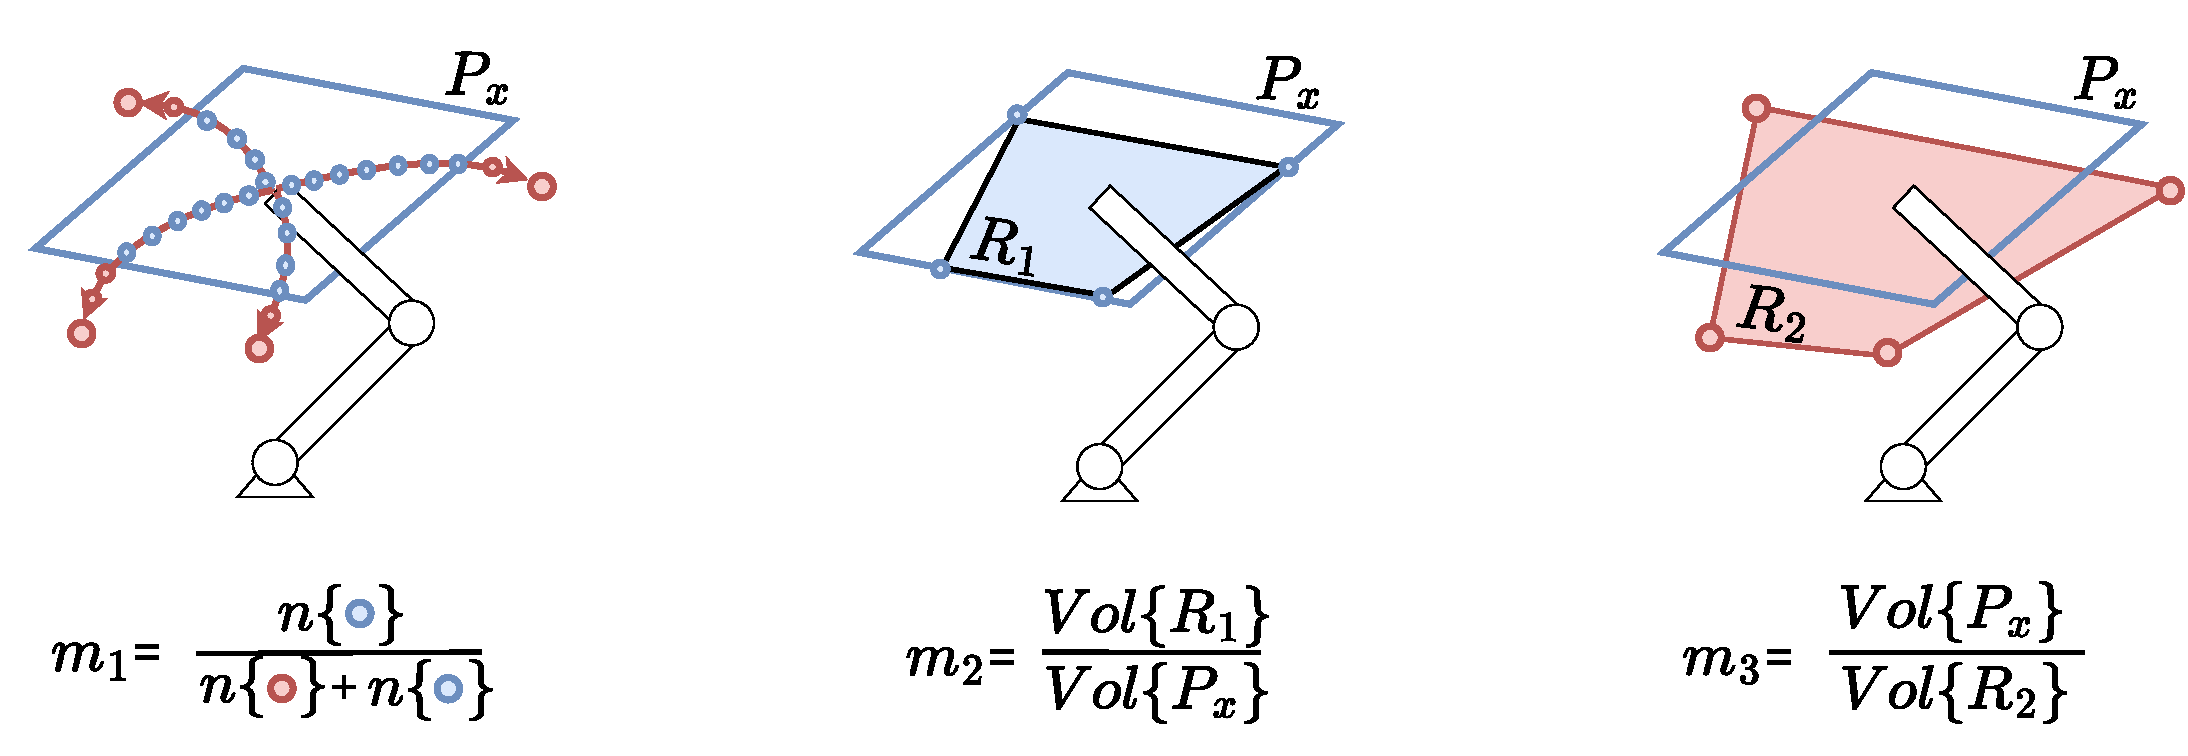
\includegraphics[width=0.8\textwidth]{Papers/images/metrics.pdf}
    \caption{Depiction of the defined quantitative metrics for a simple 2 link planar robot. The notation $n\{\cdot\}$ represents to the number of points.}
    \label{fig:metrics_defintition}
\end{figure}

\paragraph*{Metric $m_1$} First metric, $m_1$, is defined as a ratio of number of the robot's \gls{cs} positions $\bm{x}_k\in \mathcal{X}$, reached in the simulations, inside the polytope $\mathcal{P}_x$ with respect to the overall number of simulated positions. 
\begin{equation}
    m_1 = \frac{|\mathcal{X}\cap\mathcal{P}_x|}{|\mathcal{X}|} = \frac{|\mathcal{X}\cap\mathcal{P}_x|}{N\cdot n_v}
\end{equation}
The notation $|\cdot|$ represents the number of elements of the set. The metric $m_1$ gives an insight on how well the polytope $\mathcal{P}_x$ encapsulates the real reachable space determined with simulations. This metric is designed to asses the confidence in the polytope $\mathcal{P}_x$. The closer this metric is to 1, the less chance that the robot can exit the space bounded by $\mathcal{P}_x$.

\paragraph*{Metric $m_2$}  The second metric, $m_2$, is defined as the ratio of the volumes of the polytope $\mathcal{P}_x$ and the Convex-Hull of the subset of the reached points $\bm{x}_k\in\mathcal{X}$ that are inside of $\mathcal{P}_x$.
\begin{equation}
    m_2 = \frac{\vol{ \mathcal{R}_1}}{\vol{\mathcal{P}_x}},\qquad  \mathcal{R}_1 = \conv{\mathcal{X}\cap\mathcal{P}_x}
\end{equation}
The metric $m_2$ quantifies the quality of the approximation providing an insight into the ratio of the polytope $\mathcal{P}_x$ that is actually attained by the robot in the simulations. A low score ($m_2 << 1$) of this metric indicates that the large part of the $\mathcal{P}_x$ is not actually reachable.

\paragraph*{Metric $m_3$}  The third metric, $m_3$, is defined as the ratio of the volumes of the polytope $\mathcal{P}_x$ and the Convex-Hull of all the points $\bm{x}_k\in\mathcal{X}$, reached by the robot in the simulations.
\begin{equation}
    m_3 = \frac{\vol{\mathcal{P}_x}}{\vol{ \mathcal{R}_2 }}, \qquad \mathcal{R}_2 = \conv{\mathcal{X}}
\end{equation}
The metric $m_3$ gives insight about the ratio of the volumes of the polytope $\mathcal{P}_x$ and the simulated reachable space of the robot $\mathcal{R}_2$. This metric assesses the quality of the volume of the $\mathcal{P}_x$ as a metric. The further this metric from 1 the less confidence one has in the volume of the $\mathcal{P}_x$.

\subsubsection{Benchmark comparison}

\begin{figure}[!h]
    \centering
    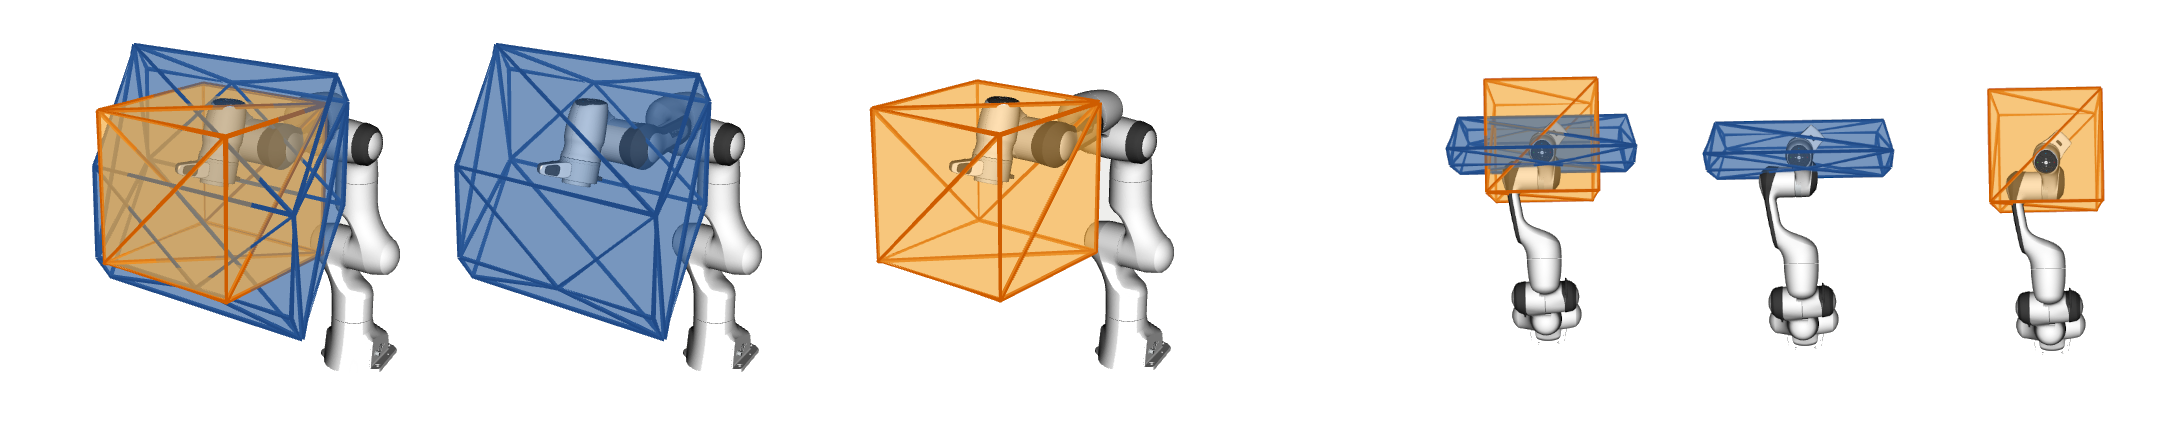
\includegraphics[width=\linewidth]{Papers/images/comp_200.png}
    \caption{Comparison of the end-effector reachable space approximation using the convex polytope $\mathcal{P}_x$ (blue) and the cube $\mathcal{C}_x$ (orange) for the Panda robot with the horizon time $t_h$=200ms. They are both evaluated in robot's initial position and the figures show two different views.}
    \label{fig:cube}
\end{figure}
To benchmark the accuracy of convex polytope approach $\mathcal{P}_x$, it is compared against the coarse approximation of the robot's end-effector reachable space using fixed \gls{cs} velocity $\dot{\bm{x}}$ and acceleration $\ddot{\bm{x}}$ limits specified by robot manufacturer.
\begin{equation}
    \ddot{\bm{x}}\in [~ \ddot{\bm{x}}_{min},  \ddot{\bm{x}}_{max}], \qquad \dot{\bm{x}} \in [~ \dot{\bm{x}}_{min},  \dot{\bm{x}}_{max}]
    \label{eq:limits_cart}
\end{equation}
The \gls{cs} limitations (\ref{eq:limits_cart}) assume that the robot's acceleration $\ddot{\bm{x}}$ and velocity $\dot{\bm{x}}$ capacity is constant. As described in \Cref{ch:robot_metrics}, this not true since the robot's movement capacity depends highly on robot's state $\{\bm{q},\dot{\bm{q}}\}$ \cite{Bowling2005}. However, the limits (\ref{eq:limits_cart}) are very convenient and widely used in many applications. A simple convex space $\mathcal{C}_x$ (cube in 3D) of reachable end-effector positions given the \gls{cs} limitations (\ref{eq:limits_cart}) can be calculated as
\begin{equation}
\begin{split}
    \mathcal{C}_x = \{ ~\bm{x}_h \in \mathbb{R}^m ~|~ \bm{x}_h &= \ddot{\bm{x}}_o\frac{t_h^2}{2} + \dot{\bm{x}}_ot_h + \bm{x}_o, \\
    \ddot{\bm{x}}_o &\in [~ \ddot{\bm{x}}_{min},  \ddot{\bm{x}}_{max}], \\
    \ddot{\bm{x}}_ot_h &\in [~ \dot{\bm{x}}_{min},  \dot{\bm{x}}_{max}] ~\}
\end{split}
\end{equation}
\Cref{fig:cube} shows the visual comparison of the two approaches: $\mathcal{P}_x$ and $\mathcal{C}_x$ calculated for one pose of the {Franka Emika Panda} robot. 

\subsubsection{Implementation details}

The proposed analysis of the reachable space polytope accuracy is performed using the numerical simulation of the collaborative robotic manipulator {Franka Emika Panda} with 7 degrees of freedom. The robot's \gls{js} limits as well as the \gls{cs} limits are taken from the manufacturer's official datasheet \cite{franka_maual}. These values are publicly available\footnote{\label{note:franka}Full datasheet available at: \url{https://frankaemika.github.io/docs/control_parameters.html}} and are listed in \Cref{tab:panda_limits_js_hfr} and \Cref{table:franka_limits_cs_hfr}.

\begin{table}[h!]
    \centering
    \begin{tabular}{|c|ccccccc|}
        \hline
        Limits & $q_0$ & $q_1$ & $q_2$ & $q_3$ & $q_4$ & $q_5$ & $q_6$ \\
        \hline
        ${\bm{q}}_{min}$ $[{rad}]$ & -2.8973 & -1.7628 & -2.8973 & -3.0718 & -2.8973 & -0.0175 & -2.8973\\
        ${\bm{q}}_{max}$ $[{rad}]$ & 2.8973 & 1.7628 & 2.8973 & -0.0698 & 2.8973 & 3.7525 & 2.8973\\
        $\dot{\bm{q}}_{max}$ $[{rad}/{s}]$ & 2.175 & 2.175 & 2.175 & 2.175 & 2.61 & 2.61 & 2.61 \\
        $\bm{\tau}_{max}$  $[Nm]$ & 87 & 87 & 87 & 87 & 12 & 12 & 12 \\
        \hline
    \end{tabular}
    \caption{Franka Emika Panda robot \gls{js} actuator limits\footref{note:franka}. The lower limits of the \gls{js} velocity and torque are symmetric to their upper limits.}
    \label{tab:panda_limits_js_hfr}
\end{table}

	
\begin{table}[h]
    \centering
    \begin{tabular}{|c|cc|}
        \hline
        Limits & Translation & Orientation \\
        \hline
        $\dot{\bm{x}}_{max}$ & 1.7 $m/s$ & 2.5 $rad/s$ \\
        $\ddot{\bm{x}}_{max}$ & 13 $m/s^2$ & 25 $rad/s^{2}$\\
        \hline
    \end{tabular}
    \caption{Franka Emika Panda robot \gls{cs} kinematic limits\footref{note:franka}. The lower limits of the \gls{cs} velocity and acceleration are symmetric to their upper limits.}
    \label{table:franka_limits_cs_hfr}
\end{table}

Robot modeling and kinematics as well as simulations of robot dynamics are built using the Python implementation of the \codet{roboticstoolbox} \cite{rtb} package. 
The evaluation of the reachable space polytope $\mathcal{P}_x$ and $\mathcal{C}_x$ is carried out using the ICHM algorithm's efficient Python implementation within the \codet{pycapacity}\footnote{\url{https://auctus-team.github.io/pycapacity/}} package, described more in detail in \Cref{ch:software}. The ICHM's approximation accuracy used for all the evaluations is $\delta$=1mm.

Eight different horizon lengths $t_h$ are chosen for the experiments
$$
t_h = [0.05s, ~ 0.15s, ~ 0.25s, ~ 0.5s,~ 0.75s,~ 1.0s,~ 1.5s, ~ 2.0s]
$$
and the simulation sample time has been set to $\Delta t$=5ms. 

The proposed method's implementation as well as the code used for the experiments is open-source and can be found in the GitLab repository\footnote{GitLab: \url{https://gitlab.inria.fr/auctus-team/people/antunskuric/reachable_space/}}. The GitLab repository additionally contains a \gls{ros} \cite{ros} implementation of the proposed method for more interactive evaluation. Furthermore, an efficient implementation of the reachable space polytope can be found as a part of \codet{pycapacity} Python package as well. All the simulations are run on a computer with 1.90GHz Intel i7-8650U processor and 32Gb of RAM memory.
 
\subsubsection{Results of the numerical analysis}
\label{ch:results}

This section brings the results of the numerical analysis of the computation time and the accuracy of the proposed reachable space approximation.

\subsubsection*{Execution time}

\begin{figure}[!h]
    \centering
    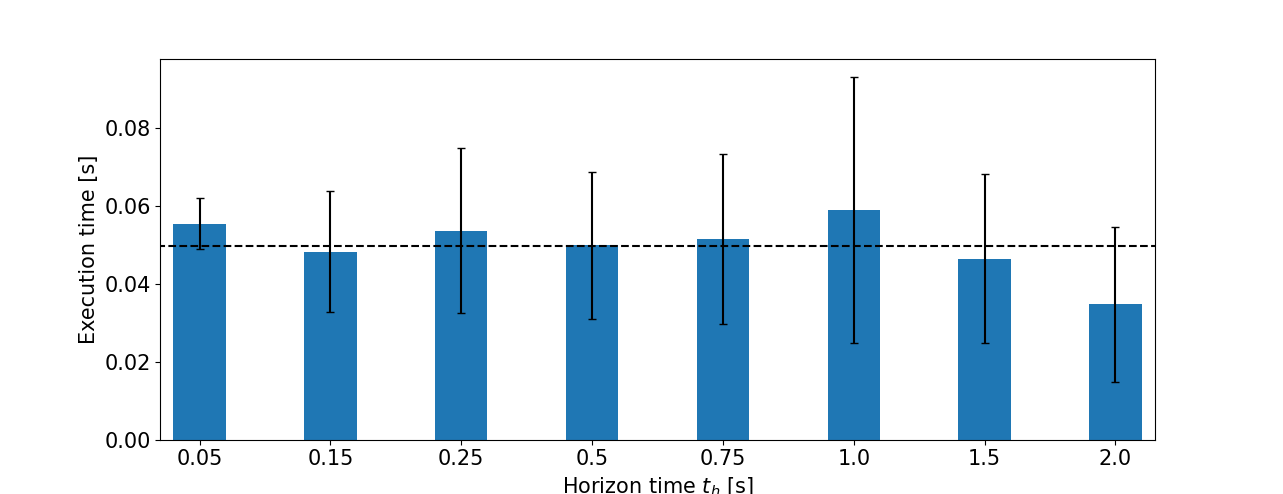
\includegraphics[width=0.9\linewidth]{Papers/images/time.png}
    \caption{Execution time of the polytope $\mathcal{P}_x$ enumeration using ICHM algorithm. Average and standard deviation calculated over 1000 executions for each of the 8 horizon lengths.}
    \label{fig:exec_time}
\end{figure}
\Cref{fig:exec_time} shows the polytope $\mathcal{P}_x$ execution time averaged over 1000 random robot configurations for each of the 8 horizon lengths. From the figure it can be seen that the execution time is relatively consistent through all the horizon lengths, with an average value around 50 ms. The constant execution time is expected because the horizon length $t_h$ does not have a big influence on the geometrical complexity of the polytope (number of vertices and faces). Rather than on the complexity, as shown on \Cref{fig:horizon}, the horizon time $t_h$ has an influence on the scale of the polytope.

\begin{figure}[!h]
    \centering
    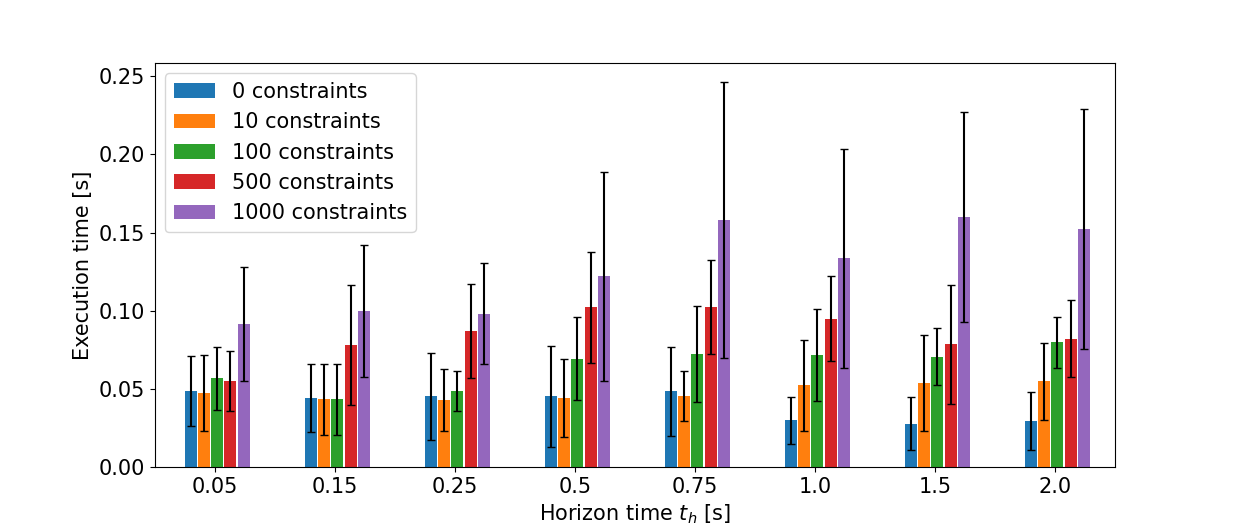
\includegraphics[width=0.9\linewidth]{Papers/images/time_constriant.png}
    \caption{Average execution time and standard deviation calculated over 1000 executions for each of the 8 horizon lengths, with different number of added environmental constraints, ranging from 0 to 1000.}
    \label{fig:exec_time_constraints}
\end{figure}
\Cref{fig:exec_time_constraints} shows the ICHM execution time for the 8 horizon lengths with different numbers of environmental constraints $A_e\bm{x}\!\leq\!\bm{b}_e$. All the environmental constraints are generated randomly and all the results are averaged over 1000 random robot configurations for each horizon length $t_h$ and all 5 different numbers of environmental constraints: 0 (no environment constraints), 10, 100, 500 and 1000. Results show that up to 10 added environmental constraints the execution time of the method does not change significantly, having the average execution time around 50ms. With 100 environmental constraints the average execution time increases around 20\% to around 70ms, for 500 the average execution is 100ms and with 1000 constraints the average execution time more than doubles, to 150ms.   


The execution time analysis of the ICHM algorithm has shown that the average polytope $\mathcal{P}_x$ enumeration takes between 50 and 150ms, which opens many doors for potential real-time applications. 

The average execution time of the nonlinear simulation for $t_h$=50ms and $\Delta t$=5ms is around 60s, and it grows to about 240s for $t_h$=2s. The cube $\mathcal{C}_x$ average execution time stays constant for all horizon lengths at around 2ms.


\subsubsection*{Accuracy analysis}

\begin{figure}[!t]
    \centering
    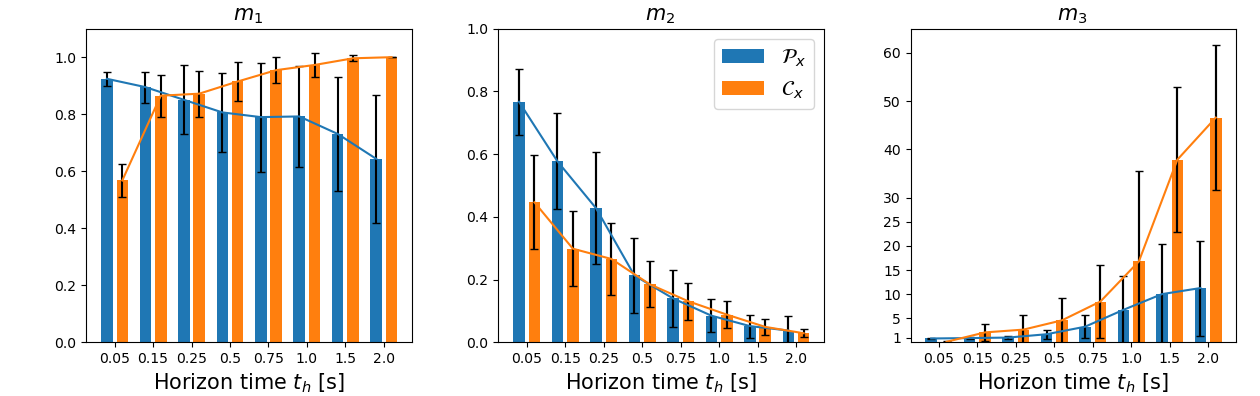
\includegraphics[width=\textwidth]{Papers/images/metrics_results_double.png}
    \caption{Accuracy measures calculated for $\mathcal{P}_x$ and $\mathcal{C}_x$, averaged over 100 random poses of the Franka Emika Panda robot for each of 8 horizon lengths.}
    \label{fig:accuracy}
    
\end{figure}
\Cref{fig:accuracy} shows the evolution of the three metrics $m_1$, $m_2$ and $m_3$ with respect to the horizon length $t_h$ for the $\mathcal{P}_x$ and $\mathcal{C}_x$, averaged over 100 random robot configurations. 

The first graph on the \Cref{fig:accuracy} shows the metric $m_1$. It can be seen that the ratio of simulated robot positions $\bm{x}_k \in \mathcal{X}$ inside the polytope $\mathcal{P}_x$ decreases with the increasing horizon length $t_h$, while it increases for the $\mathcal{C}_x$. For larger horizon lengths the robot is able to move far from the initial joint configuration $\bm{q}_o$ at the beginning of the horizon, making the assumption of linearity of the robot model, made for calculating $\mathcal{P}_x$, largely inaccurate. The approach $\mathcal{C}_x$, on the other hand, improves with the increase in horizon length, since the space bounded by the cube $\mathcal{C}_x$ increases linearly with the horizon length $t_h$, at some point it encapsulates the whole workspace of the robot. However, it can be seen that even though the ratio $m_1$ decreases, the polytope $\mathcal{P}_x$ still contains more than half ($\geq$60\%) of the simulated robot's reached positions $\bm{x}_k\in\mathcal{X}$. Finally, it can also be seen that the variance of $m_1$ increases considerably, lowering the confidence of the polytope $\mathcal{P}_x$ for longer horizons.

Evolution of the metric $m_2$ is shown on the middle graph of \Cref{fig:accuracy} . It can be seen that the volume of all the reached robot positions inside polytope $\mathcal{P}_x$ and $\mathcal{C}_x$ decreases considerably with the increase of the horizon time $t_h$. For the horizon times under $t_h\leq 0.25$s the majority ($\geq$50\%) of the reachable space polytope $\mathcal{P}_x$ has been reached by the robot simulations. However for the longer horizon times $t_h\geq0.5$s the reached volume ratio $m_2$ drops under 20\% of the total volume of the $\mathcal{P}_x$. In the case of $\mathcal{C}_x$, the majority ($\geq$50\%)  of the volume of the $\mathcal{C}_x$ is never reached by the robot for all tested horizon lengths $t_h$. 

% The right graph of the \Cref{fig:accuracy} shows the evolution of the metric $m_3$, the ratio of volumes of the polytope $\mathcal{P}_x$ and the Convex-Hull off all reached robot position in the simulation $\mathcal{R}_2 = \conv{\mathcal{X}}$. 

The right graph of \Cref{fig:accuracy} shows the evolution of the metric $m_3$. The graph shows that the volume of the polytope $\mathcal{P}_x$ and the cube $\mathcal{C}_x$ becomes several times higher than the volume of $\mathcal{R}_2$ with the increase in the horizon time $t_h$. For the horizon time of $t_h$=2s the average volume of $\mathcal{P}_x$ is 12 times larger than the volume of $\mathcal{R}_2$ and the volume $\mathcal{C}_x$ is more than 50 times larger than $\mathcal{R}_2$. At the same time the average reached volume $\mathcal{R}_1$ inside $\mathcal{P}_x$ and $\mathcal{C}_x$ consists of under 10\% of their volume (metric $m_2$), which potentially makes both polytope $\mathcal{P}_x$ and $\mathcal{C}_x$ impractical for many of applications.

However, for the shorter horizon times $t_h\leq0.25$s the ratio $m_3$ is very close to 1 for $\mathcal{P}_x$, which means that the reachable space polytope's $\mathcal{P}_x$ volume corresponds well to the actual reached volume of the robot $\mathcal{R}_2$.  \Cref{fig:comparisson_simu_convex} shows the comparison of the sets $\mathcal{P}_x$ and $\mathcal{R}_2$, for one configuration of a Franka Emika Panda robot.



Overall, this numerical analysis shows that the reachable space approximation based on the convex polytope $\mathcal{P}_x$ works reasonably well for low horizon times $t_h\leq250$ms. For longer horizon times $t_h>250$ms the assumption of the linearity of the system produces a large error in the reachable space estimation. In those cases, polytope $\mathcal{P}_x$ has volume several times higher than the real reachable space of the robot (shown by the metric $m_3$), most of which is not reachable by the robot at all (showed by the metric $m_2$). Finally, the results show that the polytope $\mathcal{P}_x$, even though a coarse approximation, has better performance across all the defined metrics then the $\mathcal{C}_x$ based on the constant \gls{cs} limits, at the same time having smaller average volume for the all the horizon times. These results remind, once again, that robot's \gls{cs} capacity is not constant and by modeling their evolution, even in a coarse manner, a substantial improvement in the estimation accuracy can be reached.




\begin{figure}[!t]
    \centering
    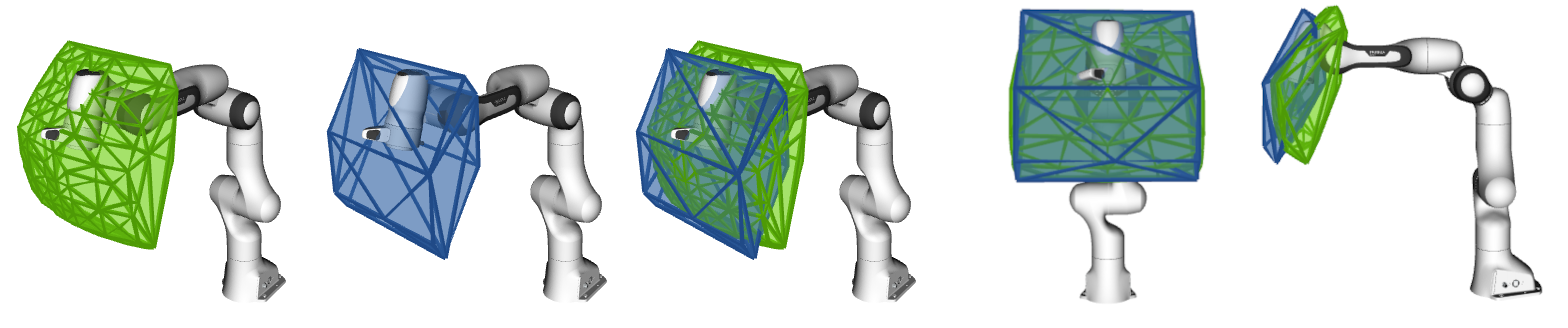
\includegraphics[width=\textwidth]{Papers/images/c3.png}
    \caption{Comparison of the end-effector reachable space approximation polytope $\mathcal{P}_x$ (blue) and the reachable space obtained using non-liner simulation $\mathcal{R}_2$ (green), from different viewpoints. Both spaces are evaluated for one robot's configuration with the horizon of $t_h=150$ms. }
    \label{fig:comparisson_simu_convex}
\end{figure}
\subsection{Discussion on limitations and potential applications}
\label{ch:discussion}

Approximating the reachable space of the robot using convex polytopes $\mathcal{P}_x$ is an efficient and relatively fast way of gaining information about the potential robot's position within the horizon of interest. Even though this approximation approach is neither an under or an over approximation of the true reachable space of the robot, as shown in the numerical analysis, for shorter horizon times $t_h\leq250$ms this metric is reasonably precise. Due to its efficiency, easy and intuitive integration of different environmental constraints, possibility to consider the robot's link geometry and the fact that its output has the form of a convex set of inequality constraints (convex polytope $\mathcal{P}_x$), it has a potential to be a useful tool for robot performance and safety analysis. However there are several important limitations of this approach.

\subsubsection{Main limitations }

First of all, the reachable space of a robot is highly non-convex and nonlinear. As shown in the numerical analysis \Cref{ch:results}, approximating this space with convex polytopes is relatively precise only for small horizon times $t_h\leq250$ms.

Secondly, robot dynamics is highly nonlinear and time variant as well. When calculating the reachable space polytope $\mathcal{P}_x$, as formulated in \Cref{ch:polytope}, the robot model is linearised in the robot's joint configuration $\bm{q}_o$ and velocity $\dot{\bm{q}}_o$  at the beginning of the horizon and this linearised model is considered constant during the horizon length. The consideration of constant robot model and its linearity, is only valid for small robot displacements around the current robot %configuration $\Delta = \bm{q}_{+1}-\bm{q}_k\approx0$
state, which is again a strong assumption and only valid for short horizon times. 

Finally, the polytope formulation from the \Cref{ch:polytope}, considers only constant joint torques $\bm{\tau}$ applied to the robot during the whole horizon length $t_h$. The polytope $\mathcal{P}_x$ calculates the joint torque vectors $\bm{\tau}$ that will produce the largest possible displacements in \gls{cs} given the robot and environment constraints. This calculation is based on the robot's linearised model at the beginning of the horizon, which in term, once again, limits the precision of the approximation to the small displacements around the initial robot state, preventing longer horizon lengths $t_h$, as confirmed in the analysis \Cref{ch:results}.



\subsubsection{Potential applications}

One promising field of applications for the polytope based reachable space metric is the human-robot interaction domain. The polytope is essentially a triangulated mesh and can be easily visualised, which could be an easy and intuitive way to give insight to the human operators about robot's real-time capabilities. This metric could potentially be used to increase human operators awareness about the robot's state during the co-manipulation by visualising the polytope $\mathcal{P}_x$ in real-time and even potentially increase the interaction safety. On the other hand, it has a potential to be used for the haptic control applications, as human operators might not be always aware of how close the robot is to the limitation of its capabilities or what is the possible space the robot can be in while teleoperating. 

Furthermore, the numerical analysis has shown that for shorter horizon times $t_h\leq250$ms the volume of the polytope $\mathcal{P}_x$ is comparable to the volume of the simulated reached space $R_2$, as shown on the \Cref{fig:accuracy}. The volume of the $\mathcal{P}_x$ could potentially be used as a performance metric for robotic workspace analysis and for applications such as robot design.

Finally, as the polytope $\mathcal{P}_x$ can be represented as a set of convex inequalities $H\bm{x}\leq\bm{d}$, this metric could potentially be used as a set of constraints for robot control. For example in case of the \gls{mpc}~\cite{Kouvaritakis2016} where, in many cases, robot's dynamics is already considered linear and constant during given horizon time, which corresponds well with the assumptions of the polytope $\mathcal{P}_x$ formulation. 

\section{Preliminary work: Non-convex approximation of the robot's reachable space}
\label{ch:curved}
One of the main limitations of the convex polytope based approach, in terms of the impact on its estimation accuracy, is the assumption of linearity of the robot's kinematics $$\bm{x} = \fk{\bm{q}_o + \Delta{\bm{q}}} \approx \bm{x}_o + J(\bm{q}_o)\Delta \bm{q}$$ throughout the horizon time $t_h$. This assumption can have an undesired effect where large parts of the polytope $\mathcal{P}_x$ can be outside of the robot's workspace, unattainable to the robot regardless of the horizon time. This is particularly noticeable in the cases where the operator is interested in visualising the robot's reachable space for longer horizon times ($t_h>0.5s$). 

Many different methods are available in the literature addressing this issue, namely in the field of robot's workspace analysis. This field brings a vast body of literature on different methods that characterise the set of the robot's reachable positions and orientations, given its actuator limits and its nonlinear kinematics, while being able to guarantee certain bounds on the approximation accuracy.
These methods are well known tools for robot design and workplace placement \cite{Gosselin1991Synthesis,kucuk2005robot}, and they are often based on Interval analysis \cite{gouttefarde2011interval} or different exhaustive sampling strategies \cite{Vahrenkamp2016}. However, as these methods are developed for the design and analysis applications, their computational efficiency does not allow for interactive applications. 

Therefore, this section brings a preliminary work on a sampling-based approach able to efficiently account for the nonlinear aspects of robot kinematics and improve the accuracy of the reachable space approximation, especially for longer horizon times. However, it is important to acknowledge that both this method and the preceding polytope approximation method lack guarantees on their approximation error.

\subsection{Sampling-based reachable space approximation strategy}

When considering a kinematic robot model in which \gls{js} velocity $\dot{\bm{q}}$ and position $\bm{q}$ adhere to constraints
\begin{equation}
   \dot{\bm{q}} \in \left[\dot{\bm{q}}_{min},\dot{\bm{q}}_{max}\right], \quad 
   \bm{q} \in \left[{\bm{q}}_{min},{\bm{q}}_{max}\right]
\end{equation}
for any given robot configuration $\bm{q}_o$ and horizon time $t_h$, the set of all the robot's reachable joint positions $\bm{q}$ can be specified
\begin{equation}
\mathcal{Q}= \{ \bm{q}\in\mathbb{R}^n ~|~ \bm{q} = \bm{q}_o + \underbrace{\dot{\bm{q}}t_h}_{\Delta \bm{q}}, \quad \bm{q}\in[\bm{q}_{min}, ~ \bm{q}_{max}],~ \dot{\bm{q}}\in[\dot{\bm{q}}_{min}, ~ \dot{\bm{q}}_{max}] \}
\end{equation}
where $\Delta \bm{q}$ represents the \gls{js} displacement from the initial position $\bm{q}_o$ during the time horizon $t_h$. As each of the $n$ components of the joint position $\bm{q}$ are independent, the set $\mathcal{Q}$ can be geometrically represented as a hyperrectangle in robot's \gls{js}.

The set $\mathcal{Q}$ (hypterrectangle) can then be transformed to the task space using the robot's forward kinematics $\fk{\cdot}$
\begin{equation}
    \mathcal{R}_x= \left\{ \bm{x} \in \mathbb{R}^m~~|~~ {\bm{q}} \in \mathcal{Q}, \quad
    \bm{x} =\fk{\bm{q}}\right\}
\end{equation}
obtaining the set of all the reachable task (Cartesian) space positions $\mathcal{R}_x$.

As a comparison, the approach described in the previous section considers the robot's kinematics to be linear during the horizon time, which yields a convex set of the task space reachable space positions that can be represented by a polytope $\mathcal{P}_x$
\begin{equation}
    \mathcal{P}_x= \left\{ \bm{x} \in \mathbb{R}^m~~|~~ \bm{q} = \bm{q}_o + \Delta \bm{q} \in {\mathcal{Q}}, \quad 
    \bm{x} = \bm{x}_o + J(\bm{q}_o)\Delta \bm{q}\right\}
\end{equation}

\begin{figure}[!h]
    \centering
    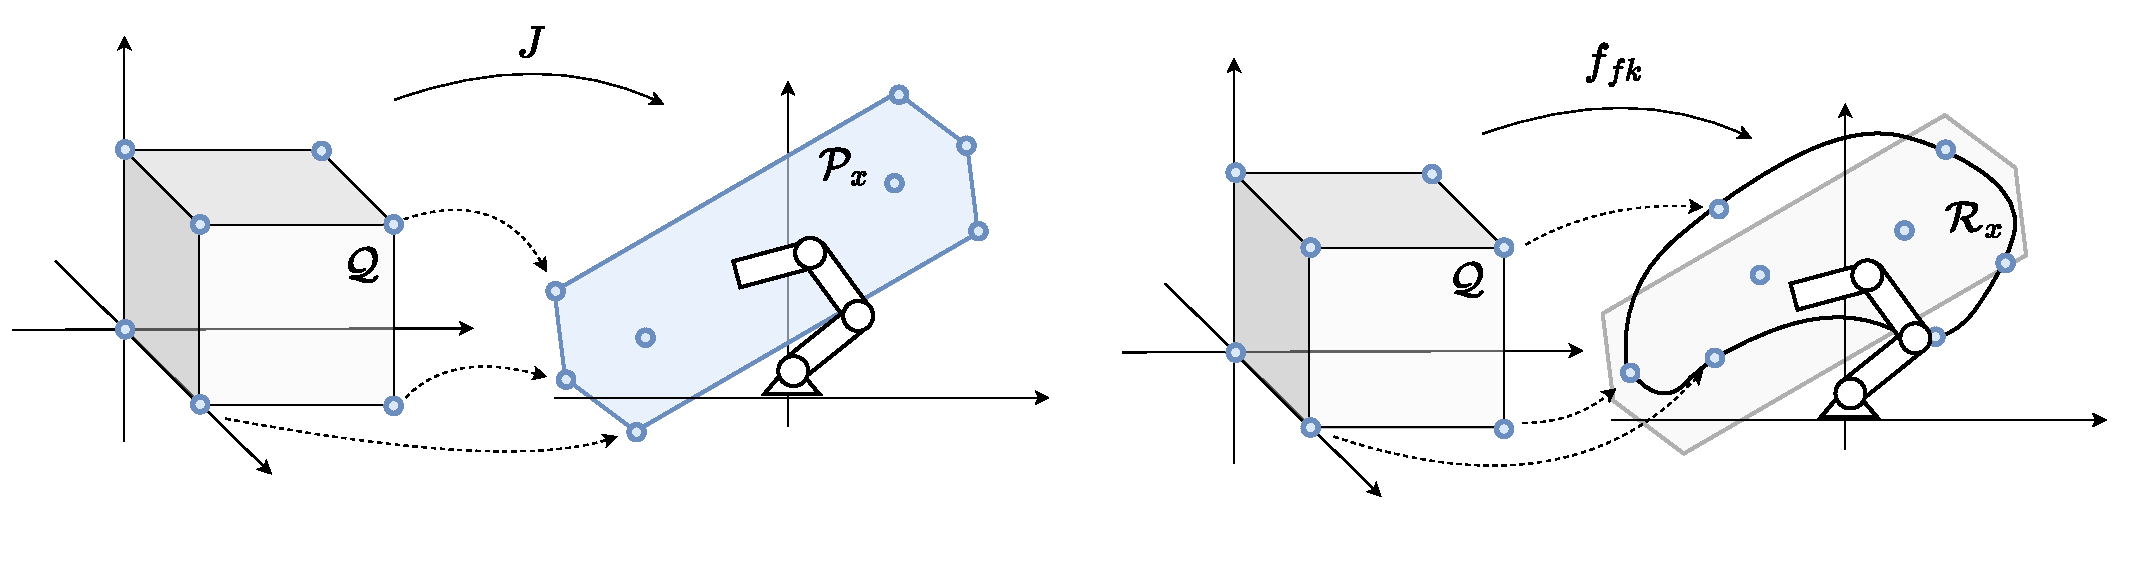
\includegraphics[width=\textwidth]{Papers/images/curved_space_algo_new.pdf}
    \caption{Simple example of the robot with $n=3$ joints and planar $m=2$ task space. The figures illustrate the difference between the linear $\mathcal{P}_x$ and nonlinear $\mathcal{R}_x$ projection of the hyperrectangle $\mathcal{Q}$ to task space.}
    \label{fig:curved_space_algo_new}
\end{figure}

\Cref{fig:curved_space_algo_new} illustrates the difference between the polytope $\mathcal{P}_x$ and the nonlinear reachable space $\mathcal{R}_x$. As shown on the figure, the polytope $\mathcal{P}_x$ is an approximation of the reachable space $\mathcal{R}_x$, which is, in general case, nonlinear and non-convex. 

Furthermore, the vertices of convex polytope $\mathcal{P}_x$ are a subset of projected vertices of the the hyperrectangle $\mathcal{Q}$. However, in the case of the set $\mathcal{R}_x$, which uses the nonlinear projection through the robot's forward kinematics, the projected vertices of the hyperrectangle $\mathcal{Q}$, are either projected to its interior or they become a part of the surfaces bounding the robot's reachable space. In general case the projected vertices are no longer the extreme points of the non-convex reachable space $\mathcal{R}_x$. 
%Therefore, as opposed to the linear approach where the projected vertices fully determine the polytope $\mathcal{P}_x$, in case of the nonlinear and non-convex space $\mathcal{R}_x$ 

\begin{figure}[!h]
    \centering
    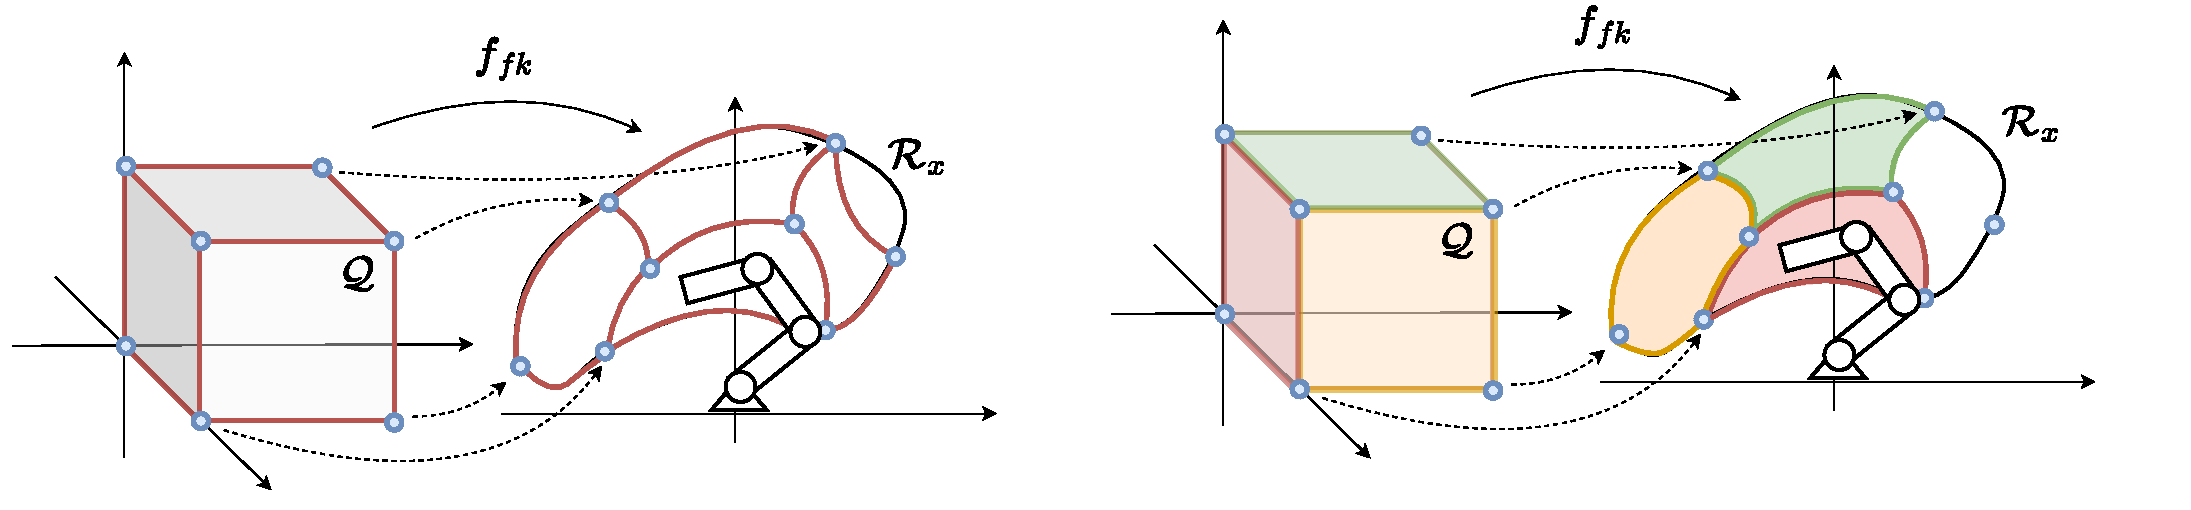
\includegraphics[width=\textwidth]{Papers/images/curved_space_algo_new_critical.pdf}
    \caption{The figures illustrate the property of the critical points to be the intersection of the $r=1$ dimensional faces and $r=2$ dimensional faces both in \gls{js} and when projected to the task space.}
    \label{fig:curved_space_algo_new_critical}
\end{figure}

These projected vertices are also called critical points \cite{MERLET1998critical}. As the forward kinematics $\fk{\cdot}$ is a continuous function, these critical points represent the intersections of the edges and faces of the set $\mathcal{Q}$ projected in the task space, as illustrated on \Cref{fig:curved_space_algo_new_critical}. Therefore, starting at any of the critical points, any other point in the space $\mathcal{R}_x$ can be reached (including the boundaries) by navigating the projected edges and faces of the set $\mathcal{Q}$. 


Leveraging this property, this work proposes a simple approximation approach of the space $\mathcal{R}_x$, based on sampling of the edges and faces of the set $\mathcal{Q}$.
This approach consists in sampling the $r$ dimensional faces ($r=0$ vertices, $r=1$ edges, $r=2$ facets, etc.) of the hyperrectangle $\mathcal{Q}$ and projecting them to the task space using the forward kinematics function $\fk{\cdot}$. This approach allows for an efficient sampling of $\mathcal{R}_x$, where its approximation can be then obtained by triangulating the obtained sample points. 

\begin{figure}[!h]
    \centering
    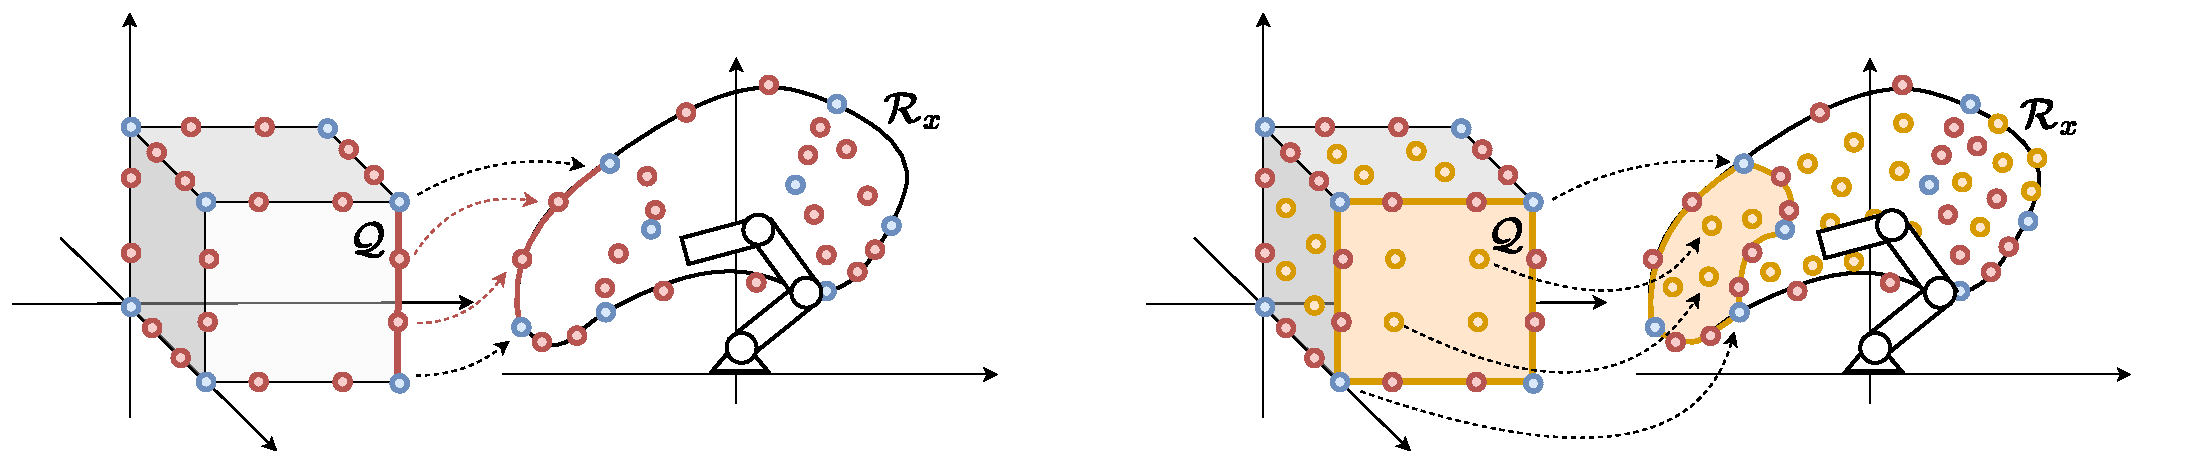
\includegraphics[width=\textwidth]{Papers/images/curved_space_algo_new_faces.pdf}
    \caption{The figures illustrate the proposed sampling-based strategy, by choosing to sample $r=1$ dimensional faces of the hypercube $\mathcal{Q}$ on the left and the $r=2$ dimensional faces on the right, while using uniform sampling with $s=4$ samples per axis.}
    \label{fig:curved_space_algo_new_faces}
\end{figure}

The proposed approach is more computationally efficient than the standard sampling methods, as it does not require sampling the complete $n$ dimensional hyperrectangle $\mathcal{Q}$, rather its $r$ dimensional faces, where $r\leq n$. \Cref{fig:curved_space_algo_new_faces} illustrates the sampling strategy. 

The proposed approach can be divided in three steps:
\begin{enumerate}
    \item Sample all the $r$ dimensional faces of the hyperrectangle $\mathcal{Q}$
    \item Project them to the task space using $\fk{\cdot}$
    \item Triangulate the obtained points
\end{enumerate}

\subsubsection*{Face dimension and sampling complexity} Determining the optimal parameters for implementation, including the dimension $r$ of the faces to be sampled and the sampling strategy, profoundly influences both the accuracy of the approximation and the execution time. These considerations are important as they describe the trade-off between approximation accuracy and time efficiency.

Increasing the dimension $r$ of the sampled faces and elevating the sampling resolution holds the potential to improve approximation accuracy. However, these improvements may come at the cost of extended execution times.

The number of $r$ dimensional faces of the $n$ dimensional hyperrectangle can be found using the equation
$$
n_f = 2^{n-r}\binom{n}{r}
$$
Moreover, in the context of uniform sampling with $s$ samples along each axis, the number of samples per $r$ dimensional face has an exponential relationship
$$
n_s = s^r
$$
As a result, the overall number of sampled points, given by $N_s = n_fn_s$, is exponentially related to the parameters $r$ and $s$. Therefore the appropriate values for $r$ and $s$ should be determined with respect to the application's requirements, in terms of the approximation accuracy and the computational complexity. 

\subsubsection*{Triangulating the non-convex space}
Furthermore, as the reachable space $\mathcal{R}_x$ is not convex, the triangulation of sampled points can be executed in multiple ways. If the application requires it, the sampled points can be triangulated using different Convex-Hull algorithms or Delaunay triangulation \cite{Lo1989Delaunay}, in order to convexify the obtained space. On the other hand, numerous non-convex triangulation methods are available in the geometric algebra, such as Alpha-shapes \cite{Edelsbrunner1994AlphaShape} triangulation. Such techniques represent better the true reachable space, but are more computationally complex. For example, in a case of a set of $n$ 3D points, the Alpha-shape algorithm's complexity is $O(n^2)$ \cite{Edelsbrunner1994AlphaShape}, while the Convex-Hull algorithms usually have a complexity of $O(n\log n)$ \cite{Barber1996}. 

\subsubsection*{Open-source implementation}
\qrimg{qrcodes/reachable_space_curved_video_sim.png}{https://youtu.be/s_bjTfJhDag}{Video}
A publicly available Python implementation of the proposed sampling-based reachable space approximation method can be found on GitLab\footnote{GitLab: \url{https://gitlab.inria.fr/auctus-team/people/antunskuric/example/reachable_workspace}} as well as a short video\footnote{Video: \url{https://youtu.be/s_bjTfJhDag}} demonstration of the method running in real-time. The implemented method uses the library \codet{pinocchio}~\cite{pinocchio2021} for robot's forward kinematics while the non-convex Alpha-shape triangulation is implemented using \codet{CGAL}~\cite{cgal3Dalpha} library.

\Cref{fig:curved_space_algo_new_real_panda} shows the visualisation of the approximation of the reachable space $\mathcal{R}_x$ using the proposed sampling method for different horizon times, while \Cref{fig:curved_space_algo_new_real_panda_curved} shows several different joint configurations for the same horizon times.


\begin{figure}[!h]
    \centering
    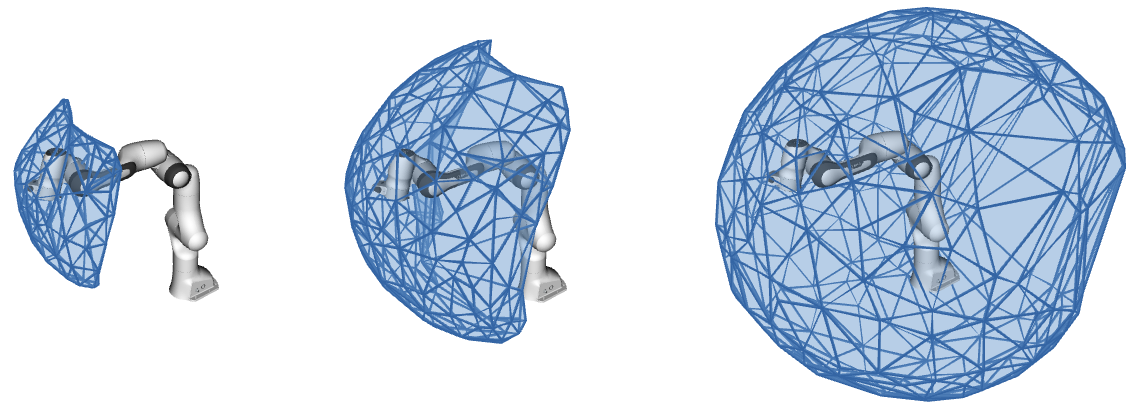
\includegraphics[width=\textwidth]{Papers/images/horizon_nonlinear.png}
    \caption{Figure showing the approximation of the reachable space $\mathcal{R}_x$ of a Franka Emika Panda robot in one configuration for three different horizon times: $t_h=100$ms, $200$ms and $500$ms (from left to right). Figures show that the approximated space is highly non-convex and for longer horizon times it tends to approach the robot's full workspace~\cite{franka_maual}.  The chosen sampling parameters are $r=3$, uniform sampling with $s=5$ and the execution time was around 500ms.}
    \label{fig:curved_space_algo_new_real_panda}
\end{figure}

\begin{figure}[!h]
    \centering
    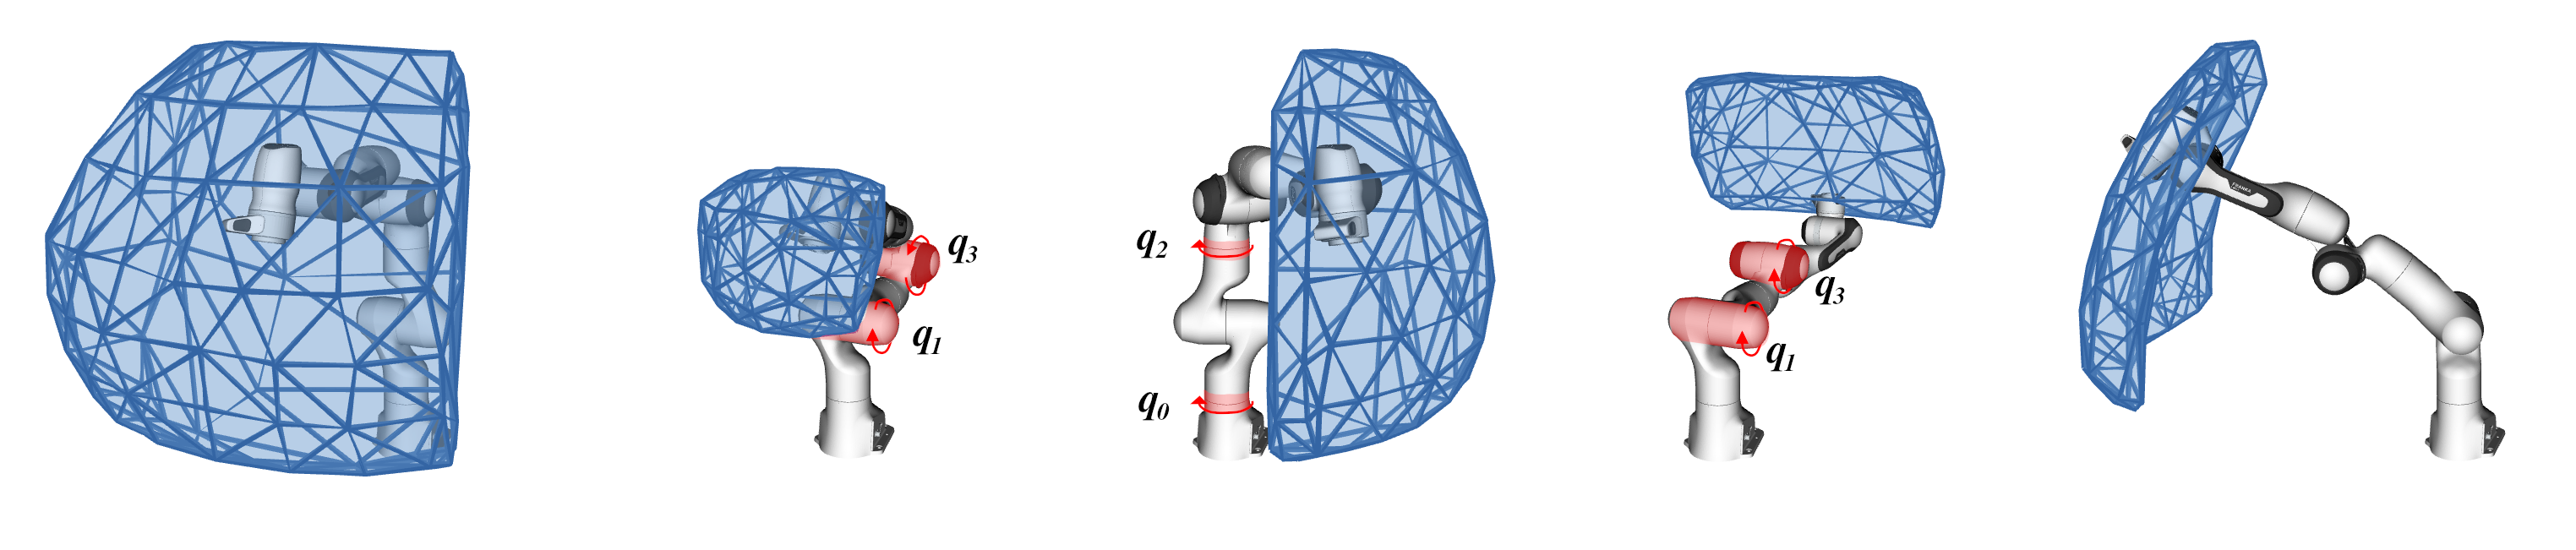
\includegraphics[width=\textwidth]{Papers/images/some_poses_robot_curved.png}
    \caption{Figure showing the approximation of the reachable space $\mathcal{R}_x$ of a Franka Emika Panda robot in five different configurations for the same horizon time: $t_h=150$ms. The first on the right shows the robot in its initial configuration, while the three following figures show the robot in configurations where two out of its seven joints are in their position limits, where the influence of robot's joint position limits can be seen through its reachable space size and shape, similar to \Cref{fig:limits}. The figure on the right, demonstrates the non-convex nature of the robot's reachable space, showing the robot in its near-singular configuration. In this configuration its movement capacity is high in tangential directions and low in radial ones. The chosen sampling parameters are $r=2$, uniform sampling with $s=3$ and the execution time was around 50ms.}
    \label{fig:curved_space_algo_new_real_panda_curved}
\end{figure}

\subsection{Discussion on limitations}

The proposed sampling-based approach holds potential for improving reachable space approximation accuracy and provide the operator with more accurate representation the robot's physical abilities. However, it has several limitations. 

The proposed method lacks formal guarantees on approximation error and, in its current form, it does not represent neither an under nor an over-approximation of the true reachable space $\mathcal{R}_x$. Furthermore, while all sampled points projected to the task space are attainable by the robot, once triangulated, the obtained space might include areas that are unattainable.

The approach's accuracy and computational efficiency heavily depends on parameter choices, like the dimension of sampled faces $r$ and the sampling strategy. Additionally, computational efficiency of forward kinematics influences overall effectiveness as well. 

Future refinements are needed to focus on addressing these limitations and to enhance the method's applicability and reliability, and in that way the quality of the information transmitted to the operator.




\section{Preliminary work: Interactive polytope visualisation platform}
\label{ch:claire}


In the context of this thesis an initial work on the development of a testing platform for the interactive visualisation of different polytopes is conducted.
The long-term aim of the testing platform is to be enable comparing different modalities of polytope visualisation to the operators and help understand and evaluate their effectiveness in different human-robot collaboration scenarios. In this preliminary work the focus is put on real-time interactive visualisation of polytopes using the \gls{ar} devices. More specifically the initial setup is built around a Microsoft HoloLens 2 device, as one of the widely used, of-the-shelf and affordable \gls{ar} devices.


% \todos{
% \begin{itemize}
%     \item development a platform for testing the visualisation of different polytope metrics using \gls{ar}
%     \item  goal to be able to test different modalities of visualising polytopes to the users
%     \item and to be able to evaluate their effectiveness within the collaboration context
% \end{itemize}
% }

\begin{figure}[!h]
    \centering
    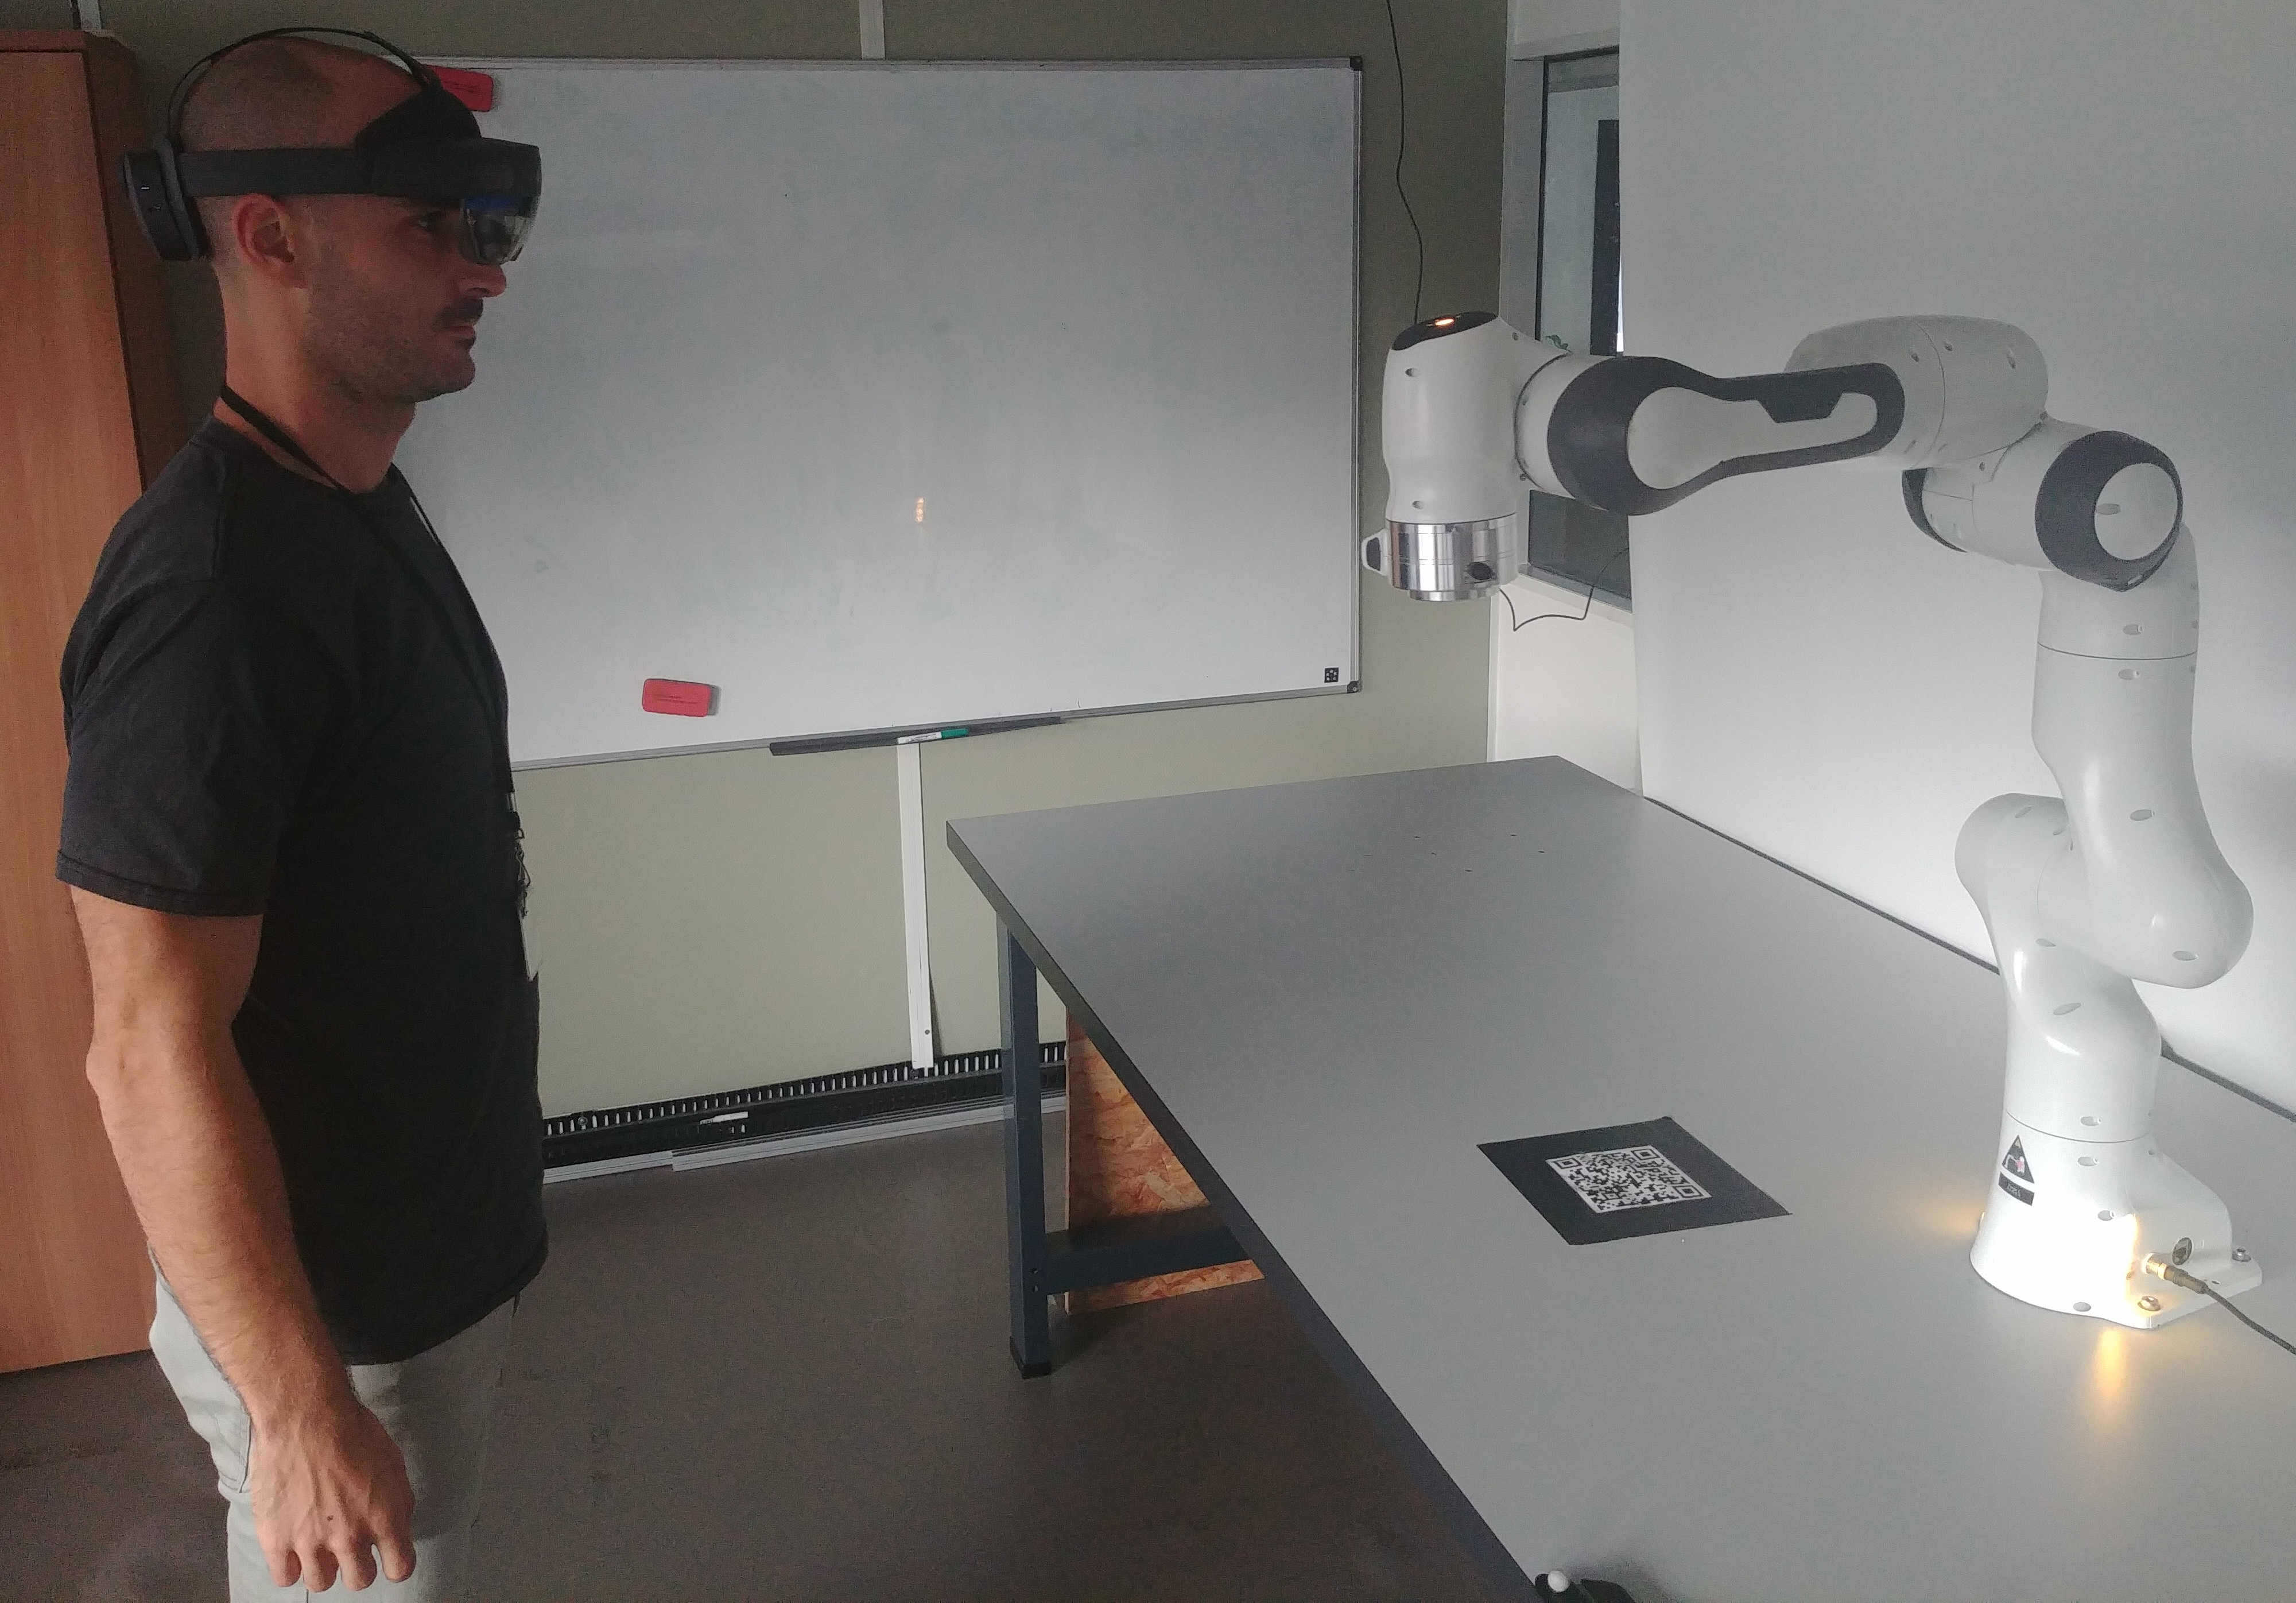
\includegraphics[width=0.39\linewidth,valign=t]{Papers/images/human_ar.jpg}
    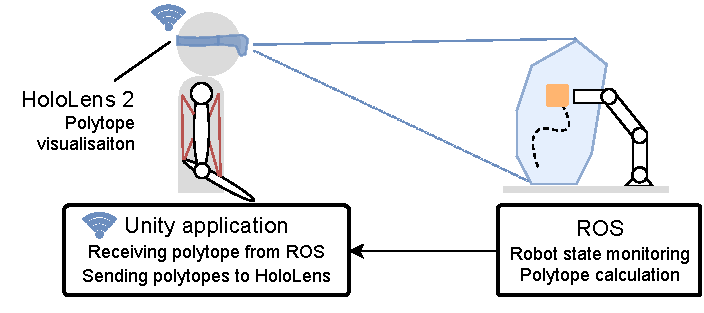
\includegraphics[width=0.6\linewidth,valign=t]{Papers/images/unity_visualisation.pdf}
    % 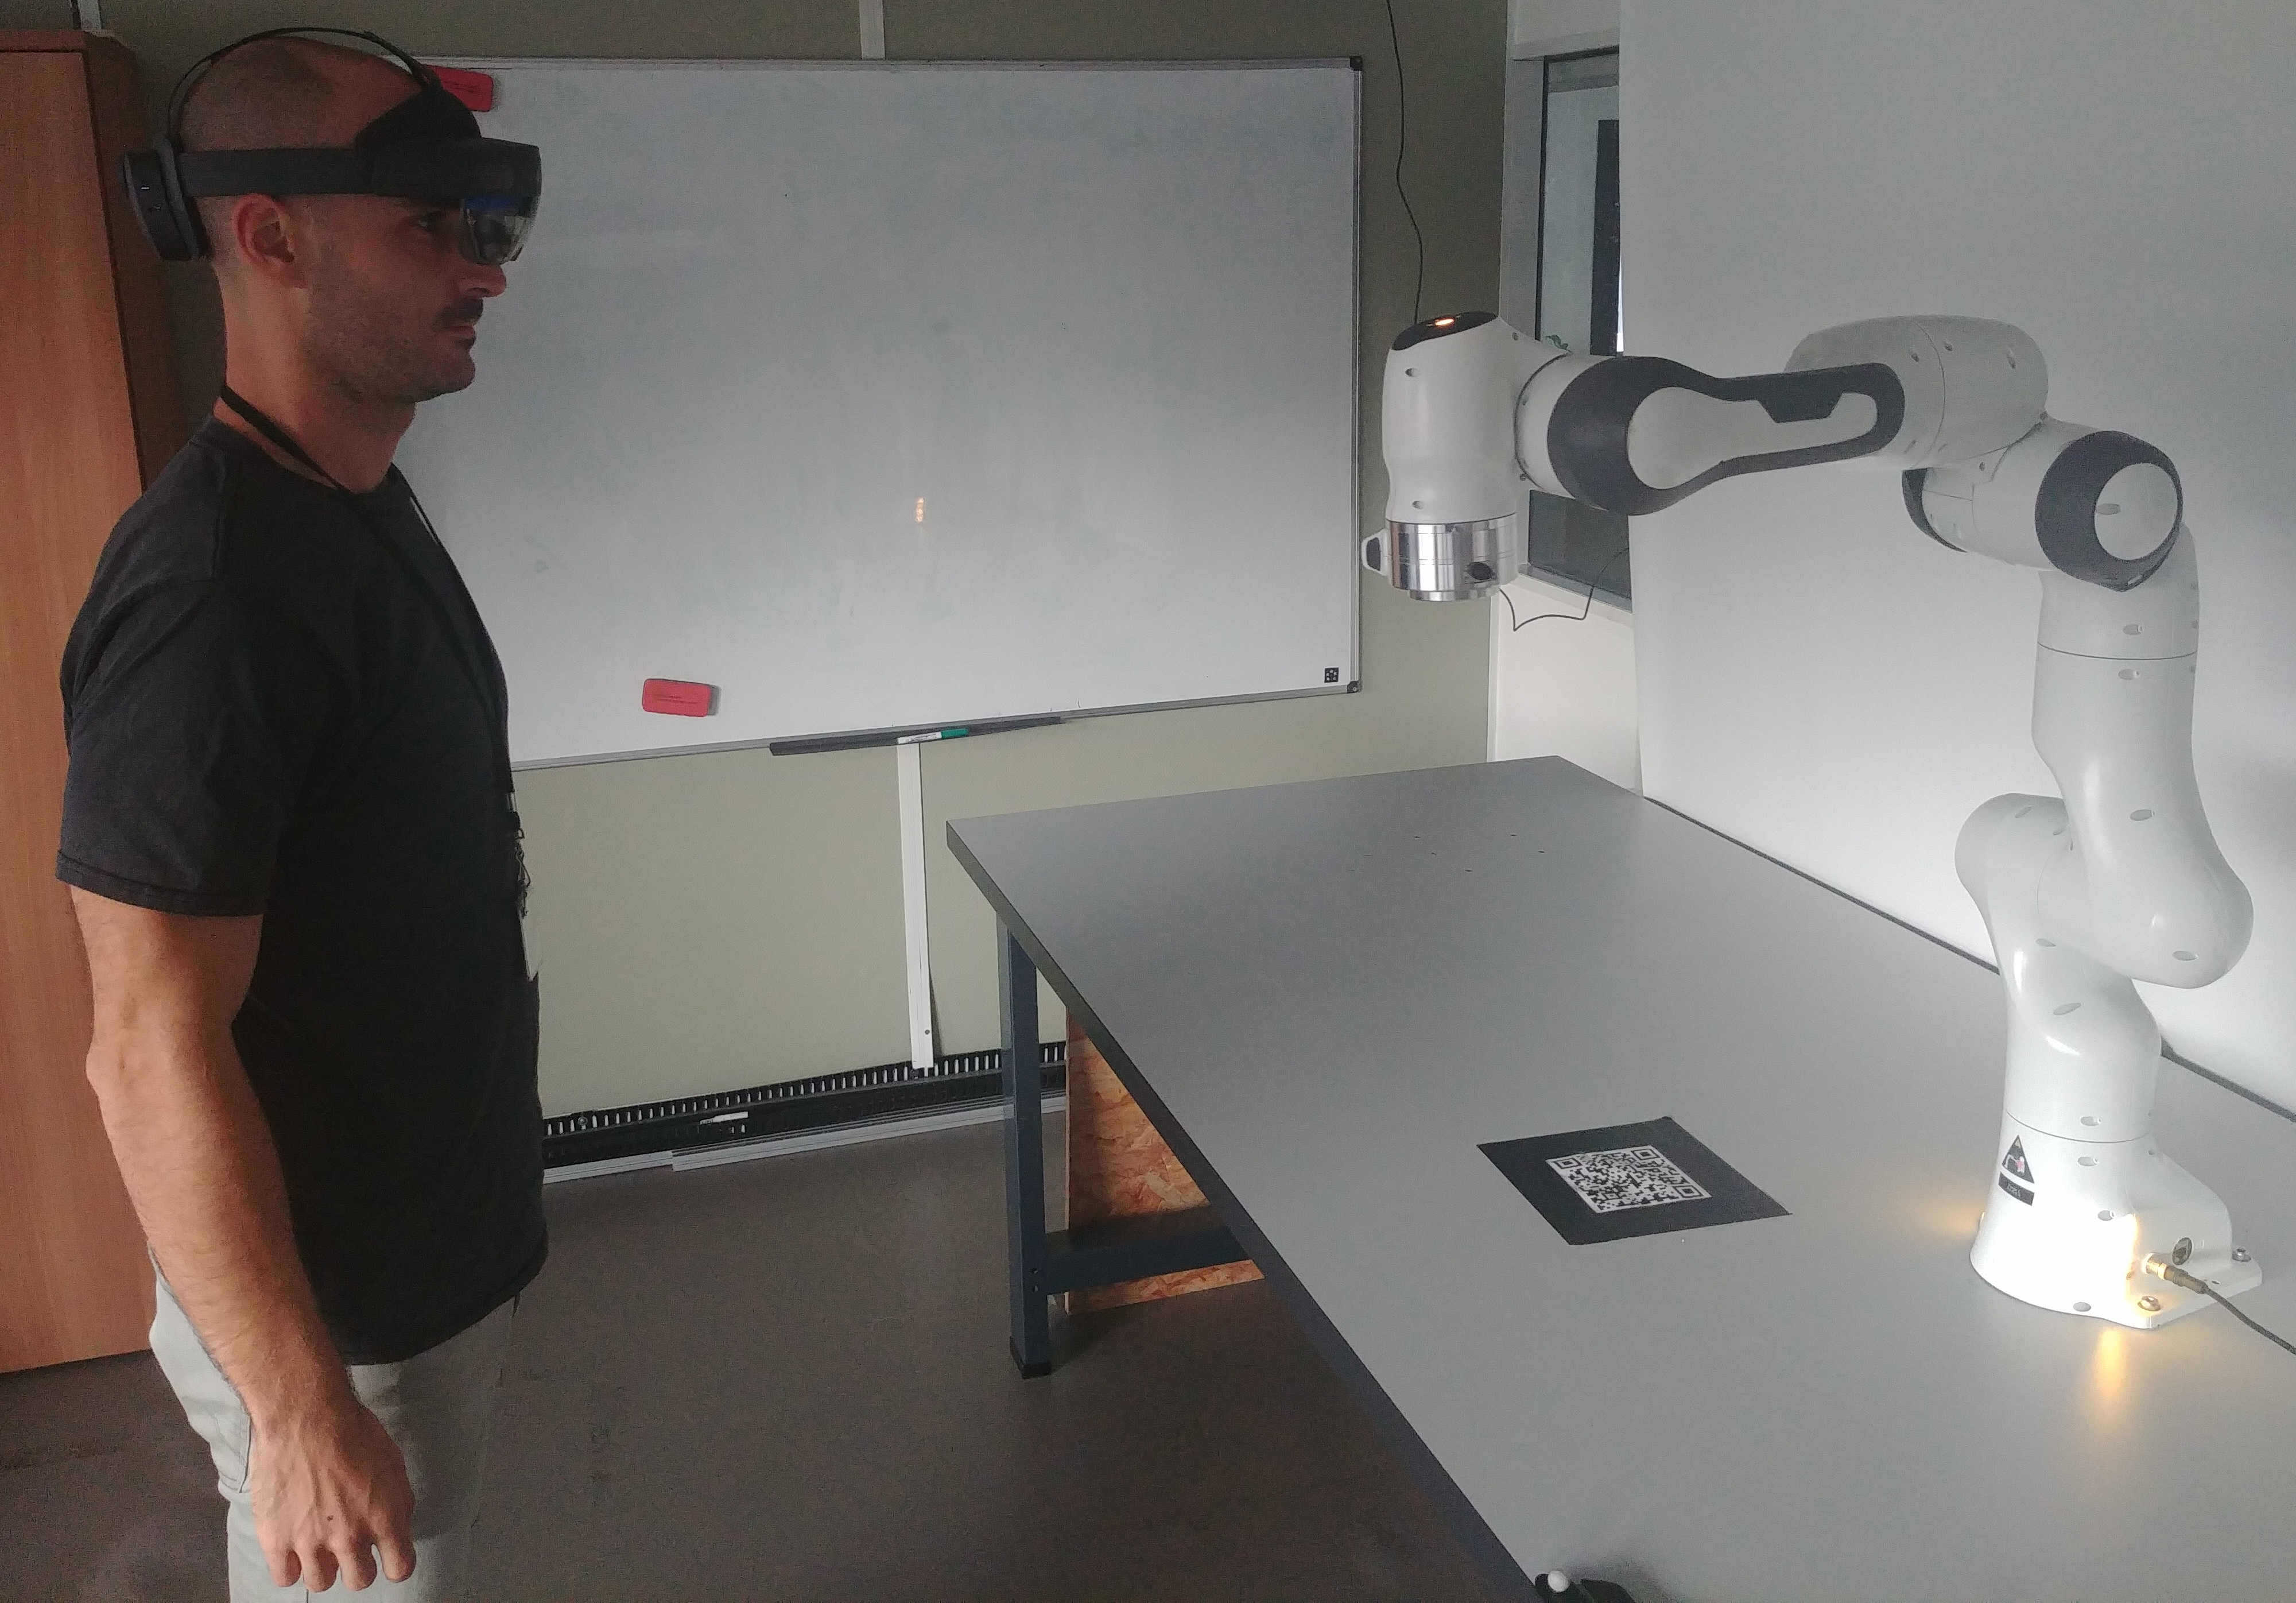
\includegraphics[width=0.55\linewidth]{Papers/images/human_ar.jpg}
    % 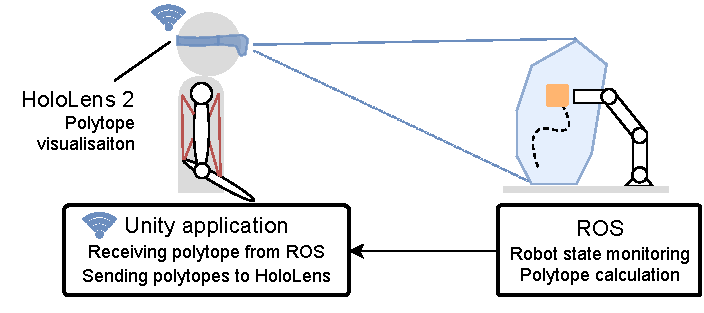
\includegraphics[width=0.75\linewidth]{Papers/images/unity_visualisation.pdf}
    \caption{Figure shows the conceptual overview of the developed platform. \gls{ros} is used to gather information about the robot's current state, which is then used to calculate different polytopes of physical abilities and prepare them for visualisation. The polytopes in form of meshes are sent to the Unity application which updates the virtual world. The updated virtual world (with polytopes) is then visualised in real-time to the operator using Microsoft HoloLens \gls{ar} headset.}
    \label{fig:unity_visual}
\end{figure}

% \todos{Maybe a paragraph stating that this work was done in collaboration with Northeastern university, or inspired by the work from \citet{Zolotas2021} or something similar.}

% \todos{
% \begin{itemize}
%     \item \Cref{fig:unity_visual} shows the proposed architecture
%     \item Using ROS to obtain robot state in real-time, pinocchio
%     \item uses pycapacity to calculate different polytopes
%     \item Sends messages to Unity ( ROS-TCP-Endpoint)
%     \item Unity app to update the virtual environment and interpret the messages 
%     \item Sends the polytopes to Microsoft HoloLens 2
%     \item Microsoft HoloLens 2 visualises the polytopes to the operator
% \end{itemize}
% }

Achieving the real-time visualisation of the physical ability polytopes with \gls{ar} devices, while making sure that the polytopes are visualised at the right place (ex. robot's end-effector), and synchronised with the robot's movements, involves several key steps. It requires real-time monitoring of the robot's state in order to calculate the appropriate polytopes and transform them to the form of triangulated meshes. The polytopes are then communicated to \gls{ar} devices, which ultimately provide the operator with the real-time interactive visualisation. 

The architecture of the implemented system is illustrated in \Cref{fig:unity_visual}. \gls{ros} is used to gather real-time data on the robot's state, while \codet{pinocchio} \cite{pinocchio2021} library is used to calculate the robot's dynamics and kinematics. The computation of various polytopes was implemented using the \codet{pycapacity} Python package. Once the polytopes are transformed to the form of triangulated meshes, they are transmitted to the Unity framework. The Unity application updates the virtual world with the new data and transmits the polytopes in real-time to the Microsoft HoloLens 2. This \gls{ar} device efficiently visualises the polytopes to the operator, at the appropriate position on the real robot (ex. robot's end-effector), providing an immersive visualisation experience for the operator.


Some components of this setup have been created through an informal collaboration with the Institute for Experiential Robotics at Northeastern University, building upon their recent work described in \citet{Zolotas2021}. Additionally, a significant portion of the platform's development has been undertaken during Claire Houziel's internship, she is pursuing her master's degree in "Robotics and Rehabilitation" at Sorbonne University.

\begin{figure}[!h]
    \centering
    % 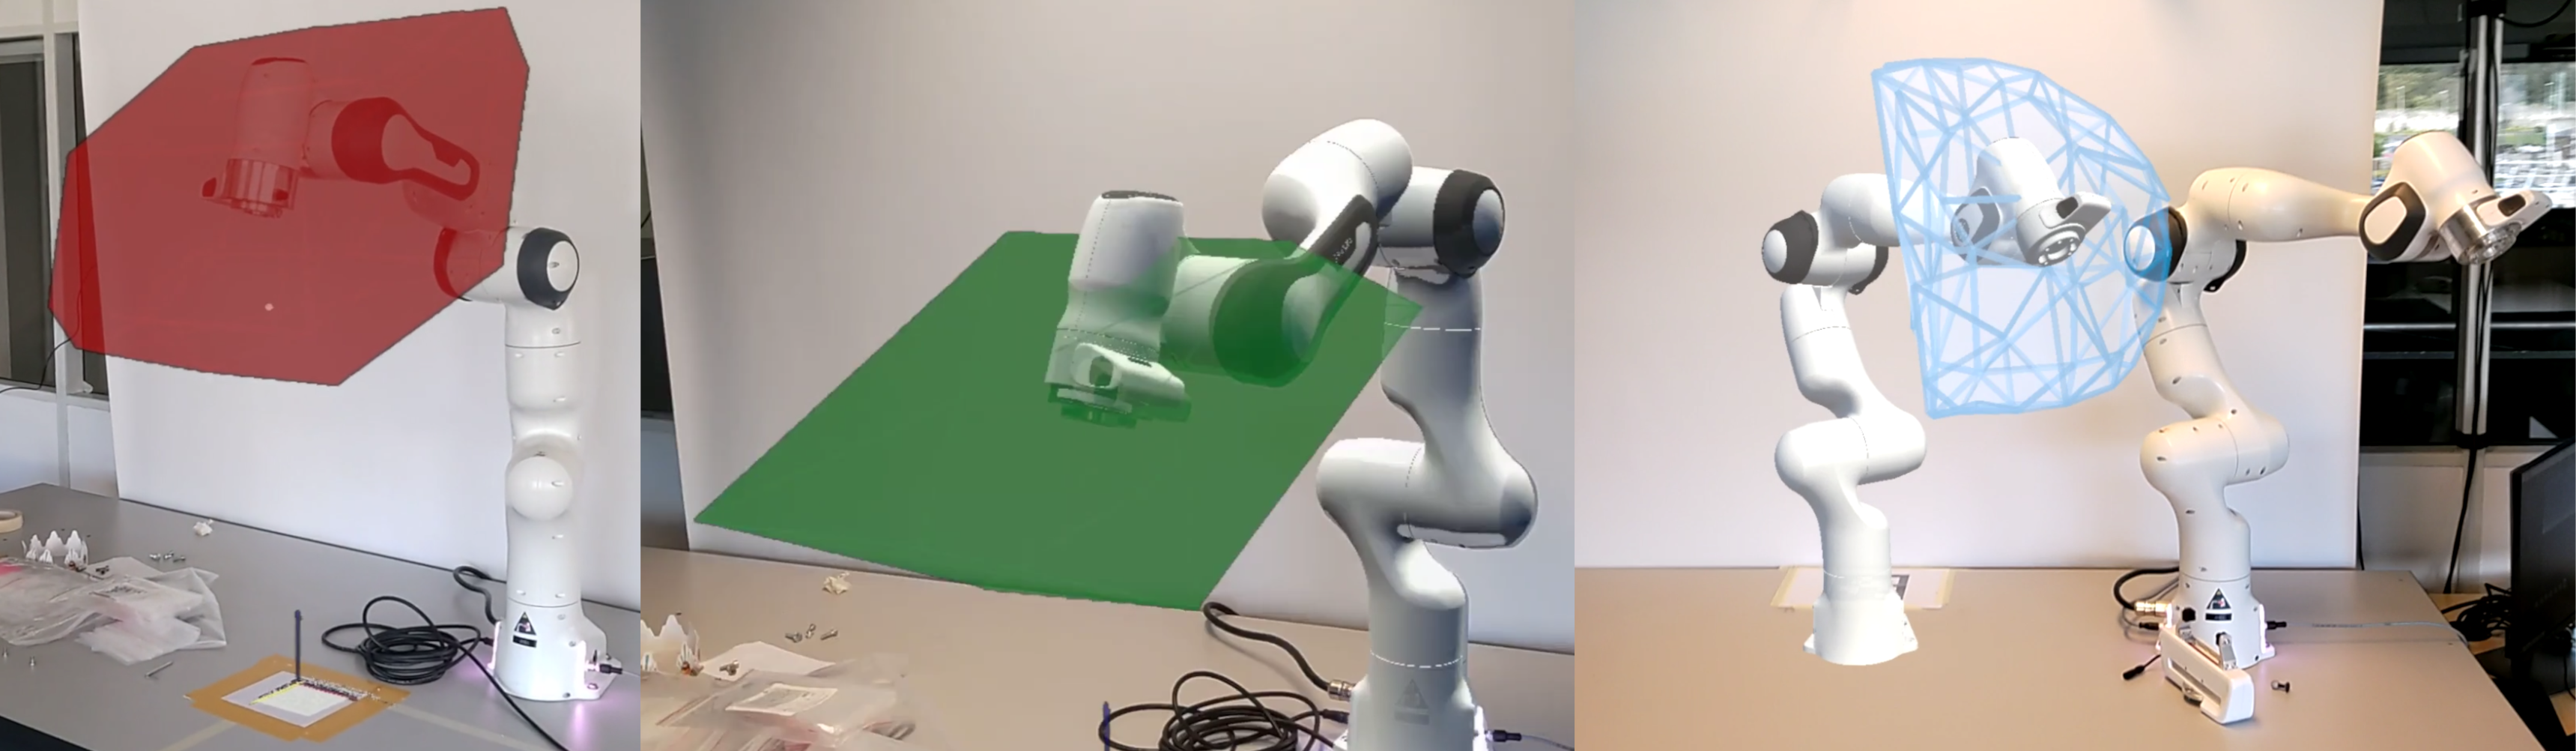
\includegraphics[width=\linewidth]{Papers/images/ar_poly_dirty.png}
    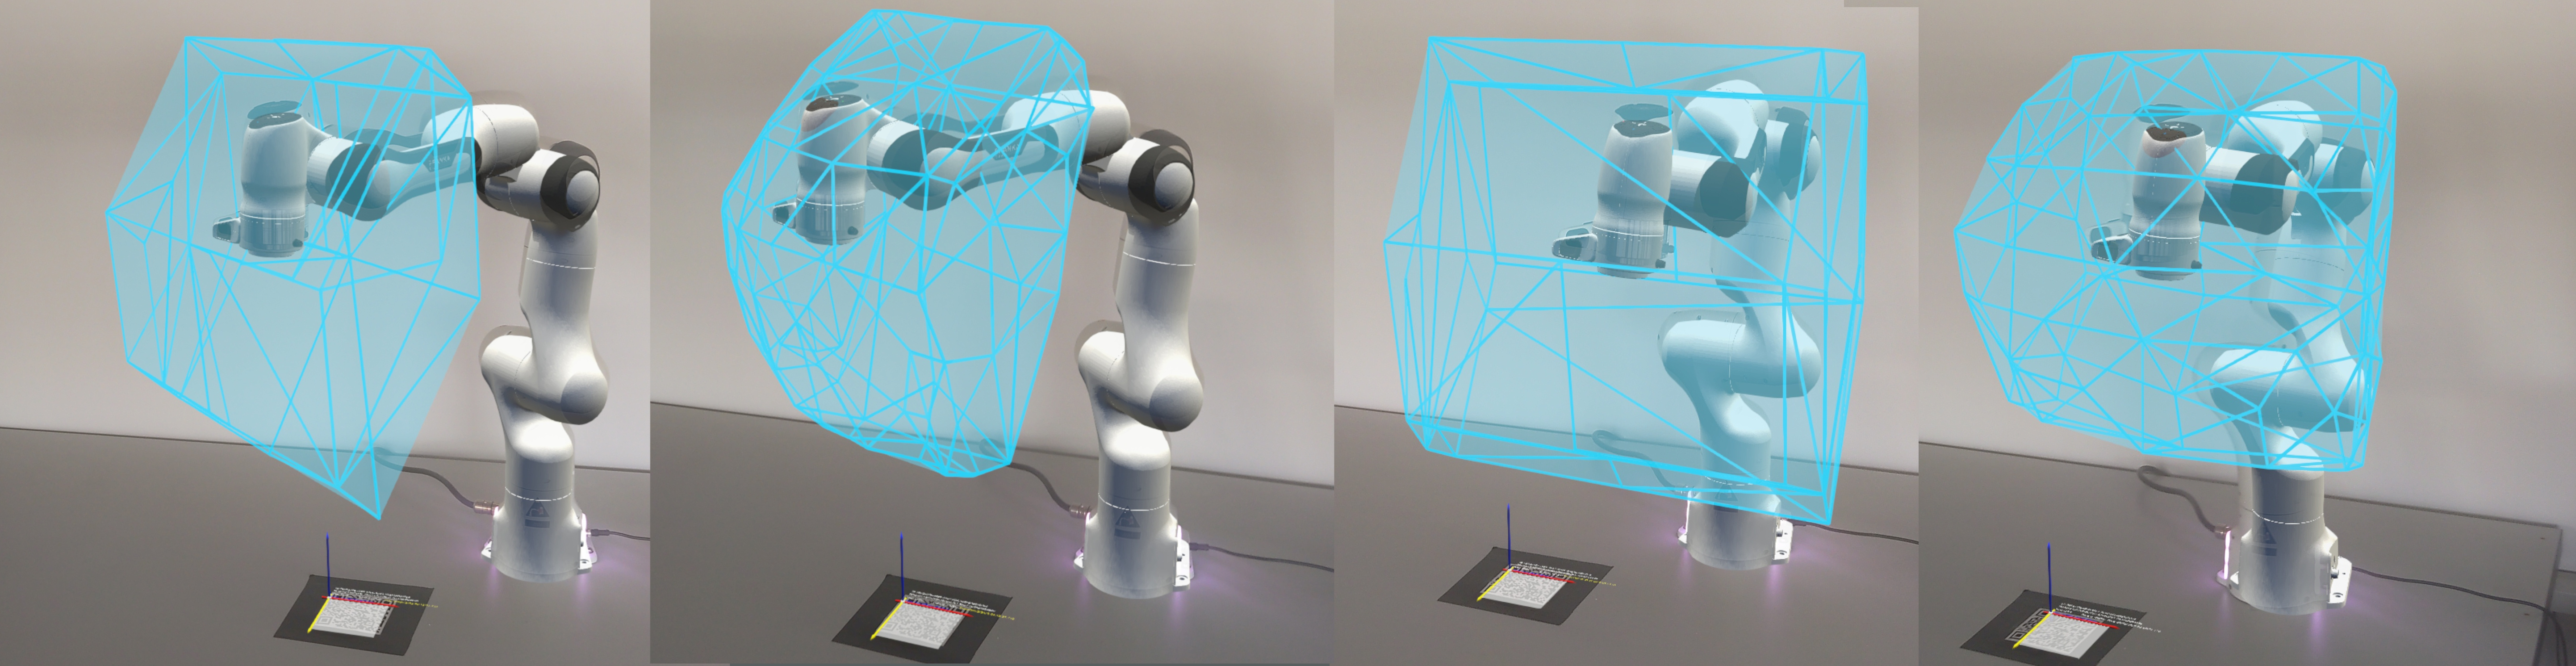
\includegraphics[width=\linewidth]{Papers/images/HoleLens3.jpg}
    \caption{Figure shows the screenshots taken from the operator's perspective using Microsoft HoloLens headset. Images show two different robot's configurations and for each one two approximations of the robot's reachable space are shown: convex polytope approach described in \Cref{ch:hfr} and non-convex approach from \Cref{ch:curved}.  
    Convex polytope is calculated with the horizon time of $t_h=200$ms, while the non-convex approximation is calculated for $t_h=100$ms.}
    \label{fig:ar_images}
\end{figure}


\begin{figure}[!h]
    \centering 
    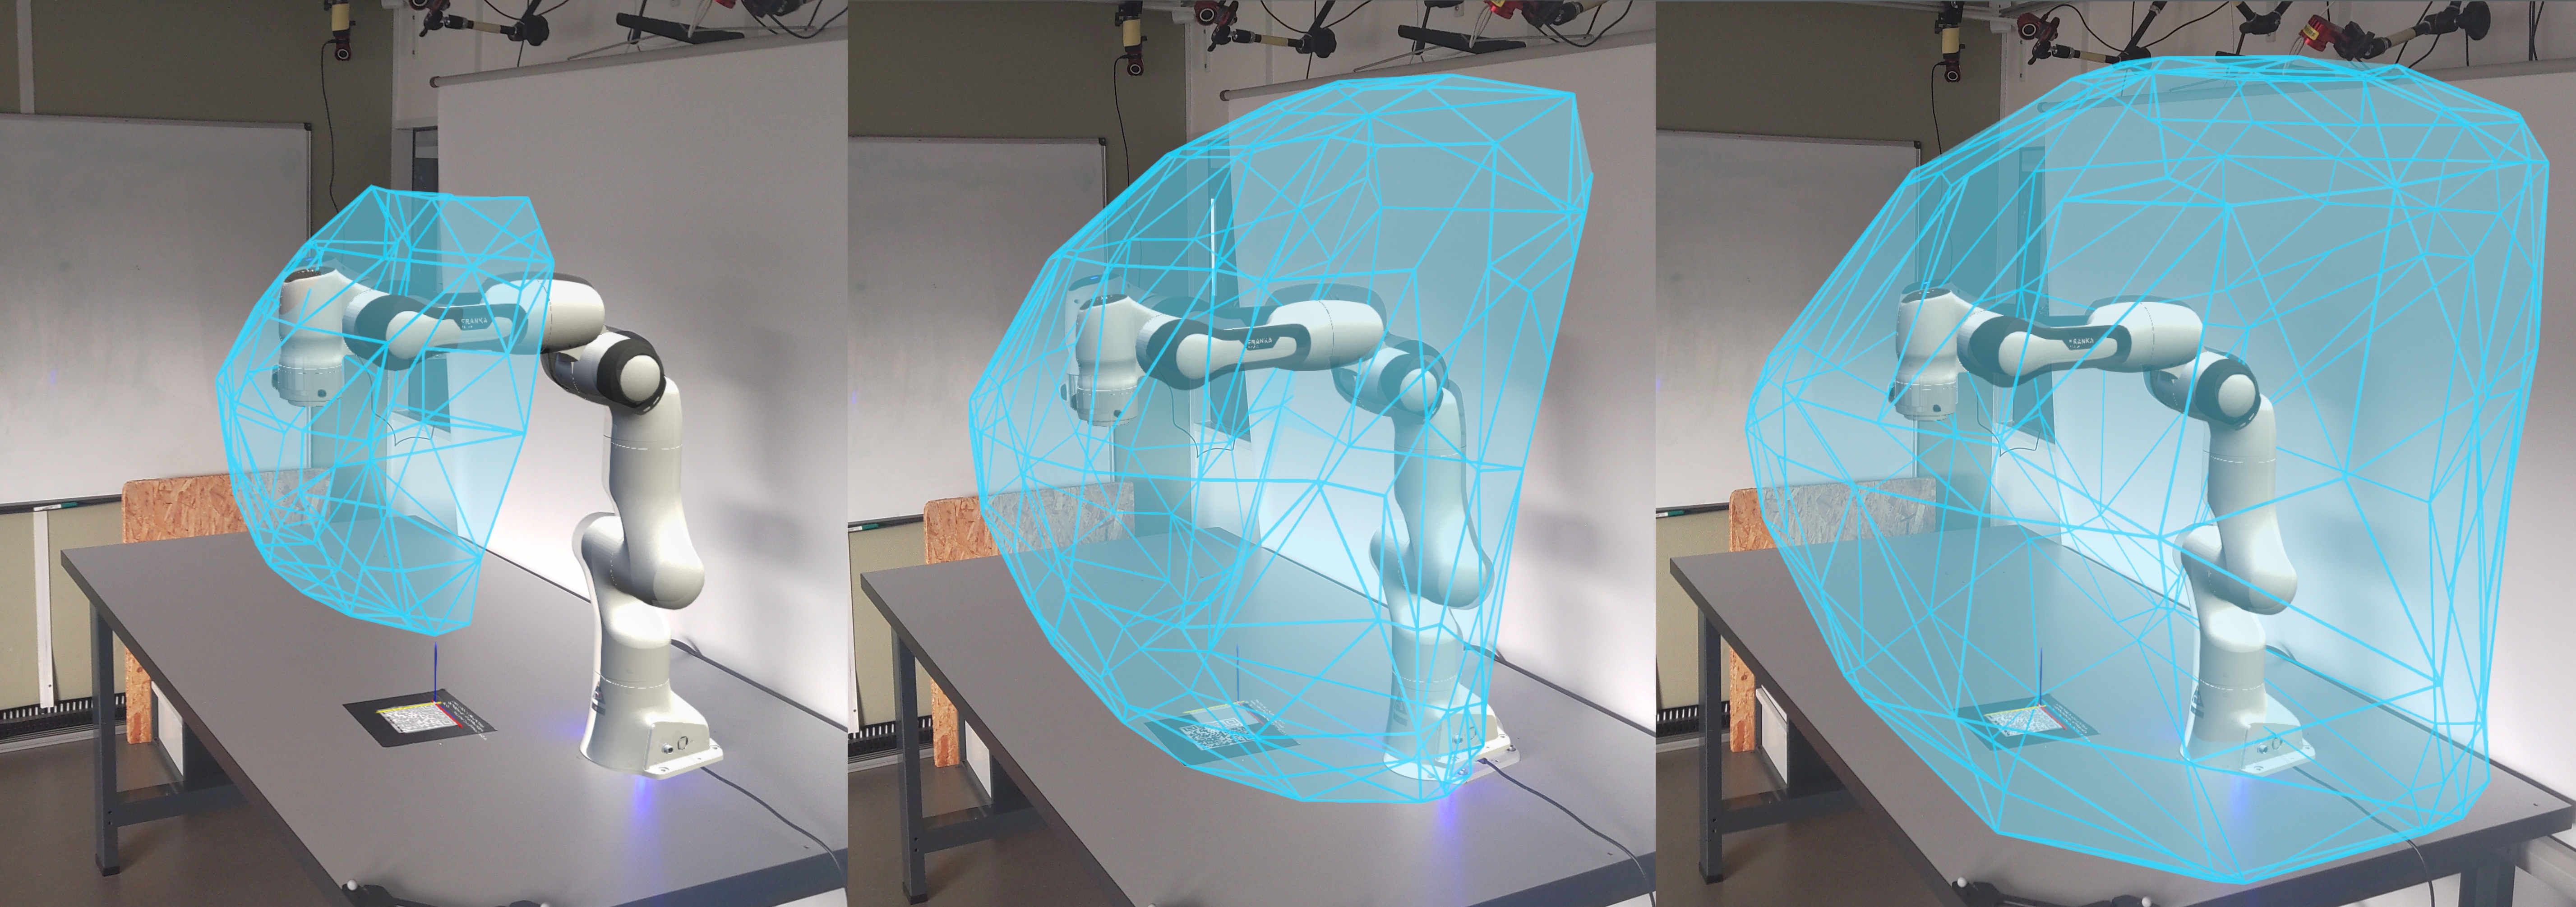
\includegraphics[width=\linewidth]{Papers/images/reachable_space_curved_ar.jpg}
    \caption{Figure shows screenshots form the Microsoft HoloLens headset. The non-convex approximation of the robot's reachable space, described in \Cref{ch:curved} , is calculated for one robot's configuration and three different horizon times $t_h=100$, $200$ and $300$ms (from left to right).}
    \label{fig:ar_images2}
\end{figure}


\qrimg{qrcodes/reachable_space_video_ar.png}{https://youtu.be/0O9b9iBzWyA}{Video}
The implemented setup allows for interactive visualisation of different polytope metrics in real-time, which serves as a base for the future work that will concentrate on the evaluation of their effectiveness for sharing information with the operator. \Cref{fig:ar_images} and \Cref{fig:ar_images2} show visualisations of several physical ability polytopes of the Franka Emika Panda robot using the developed \gls{ar} platform. Additionally, a publicly available video demonstration of the interactive visualisation of polytope metrics can be found using link\footnote{Video: \url{https://youtu.be/0O9b9iBzWyA}}.


% \begin{figure}[!h]
%      \centering
%      \begin{subfigure}[b]{0.2\linewidth}
%          \centering
%          \href{https://youtu.be/TC6r1r14FA0}{
\includegraphics[width=\textwidth]{qrcodes/reachable_space_video_ar.png}}\par \href{https://youtu.be/TC6r1r14FA0}{Video 1}
%      \end{subfigure}
%      \hfill
%      \begin{subfigure}[b]{0.2\linewidth}
%          \centering
%          \href{https://youtu.be/fscv1XtzB_o}{
\includegraphics[width=\textwidth]{qrcodes/icra2021.png}}\par \href{https://youtu.be/fscv1XtzB_o}{Video 2}
%      \end{subfigure}
%      \hfill
%      \begin{subfigure}[b]{0.2\linewidth}
%          \centering
%          \href{https://youtu.be/jTJCCn27dPk}{
\includegraphics[width=\textwidth]{qrcodes/icra2021.png}}\par \href{https://youtu.be/jTJCCn27dPk}{Video 3}
%      \end{subfigure}
% \end{figure}

\section{Conclusion}


This chapter discusses the concept of utilising polytopes as a visualisation tool to inform operators about the robot's real-time state and its changing physical capabilities. By providing dynamic and interactive visualisations of polytope based metrics, this approach holds the potential to significantly enhance operators' situational awareness. Not only enhancing operator safety by allowing them to better understand the robot's capabilities and limitations, but also having the capacity to improve overall collaboration performance. 

% \todos{
% \begin{itemize}
%     \item this chapter brings the discussion on using polytopes as a visualisaiton tool for informing the operator about the robot's current state and its current phyisical abilities. 
%     \item such real-time visualisation has a potential improve the operators' situational awareness and in that way increase their safety and potentially increase the overall collaboration performance.
% \end{itemize}
% }


Polytopes offer a convenient visualisation method due to their capacity to be transformed into triangulated meshes, a format compatible with most standard visualisation tools. Among these tools, \gls{vr} and \gls{ar} devices emerge as particularly promising platforms, offering immersive and interactive visualisation experiences. Nevertheless, the challenge lies in determining which specific physical ability polytope to present to operators and selecting an appropriate visualisation mode. This task is challenging, primarily due to the intrinsic complexity of polytopes, containing a large number of faces and vertices that may overwhelm operators' cognitive capacity when extracting pertinent information. Furthermore, the common formulations of physical ability polytopes often characterise abstract physical quantities, like accelerations or forces, which may not intuitively translate to operators' understanding once displayed. The convergence of these challenges highlights the need for careful consideration of both the choice of physical ability polytope and the visualisation mode to ensure effective communication of critical information to operators.

% \todos{
% \begin{itemize}
%     \item polytopes can be easily visualised as they can be transformed to triangulated meshes that are supported with most of the standard visualisation tools
%     \item one of the promising ones are the \gls{vr} and \gls{ar} devices, enabling immersive an interactive visualisation
%     \item however, the choice of the polytope metric to be shown to the operator and the mode of the visualisation is a challenging scientific question. 
%     \item Especially since polytopes contain large amount of information (many faces and vertices) potentially requiring higher cognitive load to extract the important information. 
%     \item additionally common polytope formulations characterise the abstract physical quantities, such as accelerations or forces, that once displayed to the operator, might not be very intuitive.
% \end{itemize}
% }

This chapter, in \Cref{ch:polytope}, introduces a novel polytope formulation for robotic manipulators, which provides an approximation of the manipulator's reachable space within a given horizon time. This polytope formulation is particularly suitable for operator visualisation, as unlike traditional polytope formulations, it represents the set of robot's reachable positions, thereby simplifying interpretation for operators. Additionally, it has the capacity to integrate actuator constraints and robot's movement capacity at the same time. Moreover, it can be intuitively extended to include the environmental constraints as well as the robot's link geometry. Finally, with the execution time of around 50ms, for standard 7dof collaborative robot, it has a potential to be used for interactive visualisation. 
However, it's important to note that this formulation relies on a linearized robot model, consequently limiting its applicability to scenarios with shorter horizon times. The analysis conducted in \Cref{ch:analysis} shows that the accuracy of the approximation significantly diminishes for horizon times exceeding 250 milliseconds. 
%While this formulation presents a valuable contribution, its constraints highlight the necessity for future work to address the limitations related to longer horizon times and nonlinear kinematic models, in order to enhance its robustness and applicability across diverse scenarios.
The proposed convex polytope approximation approach have been published as a part of a scientific article \citet{Skuric2022hfr}.

% \todos{
% \begin{itemize}
%     \item this chapter brings a new polytope formulation for robotic manipulators approximating its reachable space within a horizon time. 
%     \item it represents the reachable positions so it's easy to intepret
%     \item it integrates actuator constraints as well as it muvement capacity
%     \item it can be extended to the environmental constraints as well as the robot's link geometry
%     \item it is specifically designed for visualisation to the operator
%     \item However, the metric relies on a linearised robot model, which limits its use to shorter horizon times. The analysis has shown that the accuracy of the approximation decreases significantly for horizon times longer than 250ms. 
% \end{itemize}
% }

To enhance the approximation accuracy, particularly for longer horizon times, and to provide the operator with more accurate long-term information, \Cref{ch:curved} introduces a preliminary work on the sampling-based reachable space approximation strategy. This method takes into account the robot's nonlinear kinematics and allows the non-convex characterisation of the robot's reachable spaces. Therefore, the proposed method has a potential to offer a more accurate characterisation of robot's reachable space than the convex polytope based approach. However, like the convex polytope based approach, this strategy lacks formal guarantees on its approximation accuracy, necessitating further research to enhance reliability and information quality conveyed to operators. 

% \todos{
% \begin{itemize}
%     \item In order to improve the approximation accuracy, especially fot longer horizon times,  and provide the operator with more accuracte long-term info, this chapter brings a preliminary work on the sampling-based reachable space approximation strategy. 
%     \item it is able to account for robots nonlinear kinematics could potentially presents a more accuracte characterisation of the robot's reachable space
%     \item This approach, as the earlier approach, lack formal guarantees on their approximation accuracty and future work is needed to make them more reliable and improve the quality of such information transmitted to the operator. 
% \end{itemize}
% }
Finally, in the effort to evaluate the effectiveness of the real-time polytope visualisation to the operators, 
\Cref{ch:claire} presents the preliminary work on the development of the testing setup based on \gls{ar} tools. In the context of this thesis an initial setup is developed capable of visualising different polytopes to the operator using Microsoft HoloLens. The polytopes are visualised at appropriate location on the real-robot (ex. end-effector), updated in real-time and synchronised with the movements of the robot. This setup presents the foundation for the future work on evaluating the information sharing potential of different polytope formulations and different visualisation modalities, in the context of the human-robot collaboration.

% \todos{
% \begin{itemize}
%     \item Finally, in the effort to evaluate the effectiveness of the real-time polytope visualisation to the operators, 
%     \Cref{ch:claire} presents the preliminary work on the development of the testing setup based on the \gls{ar} tools. 
%     \item In the context of this thesis an initial setup is developed capable of visualising different polytopes to the operator using the \gls{ar} headset Microsoft HoloLens 2.
%     \item The physical abiltiy polytopes are visualised at appropriate location on the real-robot (ex. end-effector) and updated in real-time and synchronised with the movements of the robot.
%     \item This setup presents the foundation for the future work on evaluating the information sharing potential of different polytope formulations and different visualisation modalities, in the context of the human-robot collaboration.
% \end{itemize}
% }

Following chapter, \Cref{ch:topca}, proposes a new \gls{cs} trajectory planning approach exploit robot's full movement capacity, while at the same time remaining reactive to the potential changes in the environment. 
\Cref{ch:software} presents the publicly available open-source software Python package \codet{pycapacity}. The package provides the efficient implementation of algorithms for evaluating polytope and ellipsoid based physical abilities of humans and robots.
